\chapter{Systematic methodology for recycling in OS AM }
\label{Chapter.3}
\minitoc

\afterpage{
	\pagestyle{empty}
	\newpage~\newpage
	%\setcounter{page}{2}
}

\newpage
	
\section{Introduction}

	%intro 
In the chapter \ref{Chapter.2}, we characterized the performance of a representative OS 3D printer.
The obtained results allow us to confirm the relevance of these devices as  a manufacturing tool.
From this point, we can focus our attention to the material recycling issues.
And specifically,  we will focus on the polymer recycling process and the importance  of a systematic protocol development for assessing the feasibility of the recycled material to be used by OS 3D printers.

	%Intro
Nowadays, the low recycling rate of polymers is still a humankind challenge due to energy, economic and logistic issues. 
	% focusing on AM
In the additive manufacturing context, there is an exponential use of thermoplastic materials in the industrial and public open source 3D printing sector, leading to an increase of the global polymer consumption and waste generation.   
	% Problematic
However, the coupling of open-source 3D printers and polymer processing could potentially offer the bases of a new paradigm of distributed recycling of polymers as it reverses the traditional paradigm of centralized recycling of polymers which is often uneconomic and energy intensive due to transportation embodied energy.
In order to achieve this goal, a first step is to prove the recycling feasibility of the materials to be used. 

%Contribution of this chapter
The contribution of this chapter is to propose a general methodology to evaluate the recyclability of polymers used as feedstock of 3D printing machines. 
The proposed methodology is applied to the recycling study of the PLA in order to understand the evolution of the mechanical properties using fused filament fabrication (FFF).  


The reminder of the chapter is organized as follows: in section \ref{Chap-3:Polymer.Recycling.Background},  we present a polymer background explaining the main concepts  concerning the quality assessment of polymer recycled materials.  
Next in section \ref{Section:General.methodology}, the proposed methodology to evaluate the feasibility of a thermoplastic polymer recycling is presented in order to contribute to the understanding of the influence of the material physico-chemical degradation on its mechanical properties and then, on its potential distributed recyclability.  
Finally,  section \ref{Section:Application.case} shows in a detailed manner the application of the methodology to the case of PLA. 
Then, the main results of this case study are presented in the chapter \ref{Chapter.4}.

 %In sections \ref{Section:Experimental.results} and \ref{Section:Comparison.recycling}, experimental results are presented and their implications on the future recycling process discussed. To finish, in section \ref{Section:conclusions}, conclusions and perspectives for future research are presented.
%
	
	
	
	
	
	
	%(MC)Nowdays, one can observe an exponential growing need of thermoplastic material consumption in the open source Additive Manufacturing context.
	%(MC)The extrusion-based systems using fused filament fabrication (FFF) technique are by now the most adopted. 
	%Importance of new recycling paradigm: "Distributed Paradigm".
	%MCOn the other hand, the coupling of open-source 3D printers and filament extruders can potentially offer the bases of a new paradigm of distributed  recycling of polymers as it reverses the traditional paradigm of centralized recycling which is often uneconomic and energy intensive due to transportation embodied energy
	%MCHowever, the recyclability conditions at which this material could be reused are still under study.
	
	%MCThe contribution of the present paper research is twofold: 
	% Contribution related to the methodology
	%MCFirst, a general methodology to evaluate the recyclability of polymers used as feedstock of 3D printing machines is proposed.
	%Contribution related to the results 
	%MCThen, the proposed methodology is applied to the recycling study of the PLA. 
	%MC-Main results of this application contribute to the understanding of the influence of the physico-chemical degradation of the material on its mechanical properties.
	
	
	% OTHERS ELEMENTS FOR THE ABSTRACT
	
	% Goal of the paper
	%In this study, we propose firstly a methodology to evaluate the mechanical recyclability of thermoplastics.
	% Case of exemple PLA
	%The case of the Polylactic Acid (PLA), material widely used in the open-source AM context, is considered and we highlight the viability of using this recycled material in open-source 3D printers. 
	
	% Explication of our approach
	%The degradation of  mechanical and rheological properties after a number of cycles of multiple extrusion and printing processes is evaluated. 
	
	% Implications of our work
	%The characterization of recycled raw materials for open-source 3D printing has implications not only to reduce the environmental impact of polymers waste, but also it will allow us to understand the technical requirements and challenges for development of open-source filament  recycling industry sector. 
	
	% RESULTATS IN ABSTRACT 
	
	
	%Moreover, this characterization also will allow the exploration of new source of materials and new composite materials for open-source 3D printing, in order to improve the quality of products made by this technology.
	
	
	%an evaluation of the mechanical recyclability of Polylactic Acid (PLA), material widely used in the open-source AM context, in order to establish the viability of this recycled material to be used in the open-source 3D printers. The degradation of  mechanical and rheological properties after a number of cycles of multiple extrusion and printing processes is evaluated. 	
	
	
	%Bloque con introduccion general
	%Polymer recycling is a way to reduce environmental impacts of accumulation of polymeric waste materials. However, low recycling rates are often observed in conventional centralized recycling plants mainly  to the challenge of collection and transportation for high-volume low-weight-polymers in conventional centralized recycling plants.
	%As the democratization of open-source 3D printers is going forward thanks to initiatives such as FabLab environments, there is a growing interest on how to use this technology to improve the efficiency of use of raw materials.
	%% Literatura review de la que se basa mi articulo
	%Studies have been proposed in order to recycle waste polymer into open-source 3D printer feedstock. The recycling of high-density polyethylene (HDPE) issued from bottles of used milk jugs through use of an open-source filament fabricator system called RecycleBot has been evaluated. 
	
	
	
	
	%\keywords{Polymer Recycling,  PLA, RepRap, Open-Source 3D printing }
	
%\end{abstract}



\section{Polymer recycling background}
\label{Chap-3:Polymer.Recycling.Background}
%\section{Introduction}
%  PROVIDING  BACKGROUND PLASTICS
% About Plastic 
The development of polymer materials has allowed the manufacture of a wide range of low-cost, low weight, high performance products and it has become a core part of technological and societal development \parencite{Andrady2009}.
% Recycling problematic. 
However, one of the main issues is the environmental impact of plastic residues due to their longevity which can reach several decades (if not millennia) \parencite{Hopewell2009}. 
% About Plastic Industry (Not int the article)
The plastic industry is almost completely dependent of fossil oil and gas, using about 4\% of worldwide oil production which is translated in approx. 299 million metric tonnes per annum in the year 2012 \parencite{Plastics2014, Plastics2016}.  



\begin{figure}[!htb]
	\centering
	\includegraphics[width=0.8\textwidth]{Figures/Chapter-3/Recycling-Strategies.pdf}
	\caption{ Recycling strategies in industrial ecology for polymeric materials. Adapted from \parencite{Clift1997, Perugini2005} }
	\label{Chap-3:Fig.Recycling.Strategies}
\end{figure}



%  PROVIDING A BACKGROUND INFORMATION ABOUT POLYMER RECYCLING
% Intro of Polymer Recycling
In the industrial ecology for polymers, different strategies have been studied  for plastic waste management, ranging from reuse and  recycling (Mechanical, Chemical, Feedstock) until thermolysis/recovery processes as illustrated by figure \ref{Chap-3:Fig.Recycling.Strategies} \parencite{Clift1997, Hopewell2009, Al-Salem2009}.
% Definition of the recycling scenarios
They can be defined as follows \parencite{Al-Salem2009, Al-Salem2010}:

\begin{description}[labelindent=0.5cm, noitemsep]
\item[Reuse:] It covers a range of nondestructive activities that finds a second or further use for end-of-first-life solid materials \parencite{Cooper2015}.
For example, a number of detergent manufacturers market refill sachets for bottled washing liquids and fabric softeners.
However, reuse is not widely practiced in relation to plastic packaging, and in general, plastic products tend to be discarded after first use \parencite{Hamad2013}.
	
\item[Mechanical recycling] It is the process in which discarded plastic is used in the manufacturing of plastic products via mechanical means, using recyclates, fillers and/or virgin polymers  \parencite{Fisher2004, Hopewell2009, Al-Salem2009, Perugini2005}.
	% Describing the process
	This process include phases such as the separation of polymer types, decontamination, size reduction, remelting and extrusion into pellets \parencite{Lazarevic2010}. 
	
\item[Chemical recycling:] Chemical recycling is a term used to refer to advanced technology processes which convert plastic materials into smaller molecules, usually liquids or gases, which are suitable for use as a feedstock for the production of new petrochemicals and plastics \parencite{Al-Salem2009}.
	
\item[Feedstock recycling:] The category refers to the recycling technologies that breaks down the solid polymeric materials into a spectrum of basic chemical components.
These processes involve the use of high temperatures to cleave the bonds in the backbone of the polymer; they can be carried out in the absence of air (pyrolysis), in the presence of a high partial pressure of hydrogen (hydrocracking), or of a controlled amount of oxygen (gasification) \parencite{Perugini2005}.

The main advantage of feedstock (and chemical) recycling is the possibility of treating heterogeneous and contaminated polymers with limited use of pre-treatment \parencite{Al-Salem2009}.


\item[Energy recovery:] This category encompass the combustion processes in order to recover the energy value of products after their useful life. 
They are used if wasted material cannot be mechanically recycled because of excessive contamination, separation difficulties, or polymer property deterioration \parencite{Perugini2005}.
Modern energy recovery facilities burn solid wastes in special combustion chambers, and use the resulting heat energy to generate steam and electricity \parencite{Subramanian2000}.

\item[Landfilling:] It is the conventional approach to waste management where disposal are discarded in an open area.
A major drawback to landfills from a sustainability aspect is that none of the material resources used to produce the plastic is recovered—the material flow is linear rather than cyclic \parencite{Hopewell2009}.

\end{description}


% Justification of Recycling approaches Vs. Others 
%Importance of  Mechanical recycling process
From the energy and environmental perspective, the research works of \textcite{Arena2003,Perugini2005,Piemonte2011} have highlighted that mechanical recycling process has been identified as the most suitable  recovery route for relatively clean and homogeneous plastic and bioplastic waste streams with respect to landfilling or incineration options.  
% %  PROVIDING  BACKGROUND OF MECHANICAL RECYCLING
% Focus on Mechanical Recycling
In particular, they showed the suitability of mechanical recycling which entails the production through physical means of new plastic products from plastic waste. 
%  Difficulties of Mechanical recycling 
However, the  difficulties of this process are mainly related to the degradation of recyclable materials,  heterogeneity of plastic wastes and the related  logistics  to the process \parencite{Al-Salem2009}.
% Justification of the difficulties of mechanical recycling
% Usa
Indeed, in U.S. only 6.5\% of the used plastics are recycled in conventional centralized recycling process \parencite{Themelis2011}. 
%  Case Europe
In Europe, only 26\% (equivalent to 6.6 million tonnes in 2012) of post-consumer plastic wastes were recycled \parencite{Plastics2014, Plastics2016}.  
% Reasons for Low mechanical recycling process
The low recycling rates could be explained by factors such as the price variation of the recycled material (due to uncertainty of petroleum supply and the cost associated),  the lower mechanical properties of the recycled polymer compared with virgin polymer, the associated  cost of recycling process (collection, sorting  and transportation).
 % Conclusion of economical point
In fact, one of the main drawbacks  is that there is no net economical benefit from recycling plastic materials  \parencite{Craighill1996}.  
%		% Availability
%Lack information about the availability of recycled plastics. 
%		% Limited knowledge
Moreover, the limited scientific knowledge about the influence of recycling processes on the composition, structure, and properties of polymeric materials makes difficult for an industrial segment of polymer recycling, to compete with the manufacturers of virgin polymers.
Indeed,  the quality properties of the virgin synthesized materials can be assessed reliably  and it is possible to define the suitability for specific applications. This is not the case for recycled material  \parencite{Hopewell2009, Vilaplana2008}.
% Conclusion of the polymer recycling problem
These general bottlenecks restrict the effective implementation of recycling activities.


% Focus on Mechanical Recycling
We will focus on the mechanical recycling process taking into account that the other recycling processes (chemical, feedstock, recovery) are not in the same order of magnitude that we are exploring.
	% Details of the mechanical process
One important element to consider in mechanical recycling process is the heterogeneity and compatibility issues of the polymers.
The more complex and contaminated the waste is, the more difficult to perform the process is.
	
	\begin{figure}[H]
		\centering
		\includegraphics[width=0.8\textwidth]{Figures/Chapter-3/Materials-methods/Process-reference/mechanical-recycling.pdf}
		\caption{Mechanical recycling steps (Adapted from \parencite{Aznar2006, Al-Salem2009} ) }
		\label{Fig:Mechanical.recycling.steps}
	\end{figure}
	
		
% Describing the stages of mechanical recycling process
Figure \ref{Fig:Mechanical.recycling.steps} provides  the usual steps involved in the mechanical recycling process \parencite{Aznar2006,Hopewell2009}.
	% Introduction to the phases
Three general phases have to be considered.
	%Phase of preparation of recycled material
In the first phase ``Preparation of the recycled material'' the material is conditioned through different steps to prepare it for the extrusion process. 
% Cost of the first phase
Being a costly and energy intense process, mechanical recyclers try to reduce these steps and working hours as much as possible \parencite{Al-Salem2009}. 
	% Phase of mouding and final product
Once the material is prepared, a plastic molding technique (e.g. extrusion, injection...) is used in order to prepare a final product. The final product could be a product made of virgin/recycled compounding or a type of recycled pellet that could be used in other manufacturing process  \parencite{Briassoulis2013}. 
%In this preliminary study we don't have to consider the first phase (\ref{mechanical.recycling}). 
%Within the framework of the present project virgin monomaterial polymer was considered as the initial feedstock of the process at the first recycling process. Because the initial properties of the material are well known, the preparation phase is not considered for the first recycling cycle.   

% Literature of Polymer Degradation
In the scientific literature, the modeling of the life cycle of recycled products is an usual approach  to investigate the mechanisms and effects of the degradation processes to which recycled products are exposed.
% Introduction of the Polymer degradation
Polymeric materials are exposed to \textit{thermo-mechanical} and \textit{thermo-oxidative} degradation \parencite{Vilaplana2008}.
% Thermo-mechanical degradation
Thermo-mechanical degradation occurs in its processing where high shear forces and high temperatures can caused chain scission and chemical reactions.
% Thermo-oxidative degradation
On the other hand, thermo-oxidative degradation can produce physical and chemical changes in the polymeric structure due to exposure of specific environmental conditions during service life. 
% Implications of the two type of degradations
Thermo-mechanical and thermo-oxidative degradations are the responsible for changes in structural and morphological characteristics of the polymers such as mechanical-rheological-thermal properties, degree of crystallinity, viscosity, and molecular composition \parencite{Vilaplana2008}.
% Importance of evaluate la degradation of polymer
This information can be used  as quality assessment of the recycled material, and also, it can also provide important inputs about the control of the processing conditions/parameters during recycling process. 
%  Exemplo of the degradation processes
The methodological approaches to investigate the  thermo-mechanical and thermo-oxidative degradation are illustrated in the \ref{Chap-3:Fig.Modelling.Life.Cycle.Recycled.Polymers}:

	\begin{figure}[H]
		\centering

\begin{subfigure}[t]{0.49\textwidth}
			\centering
		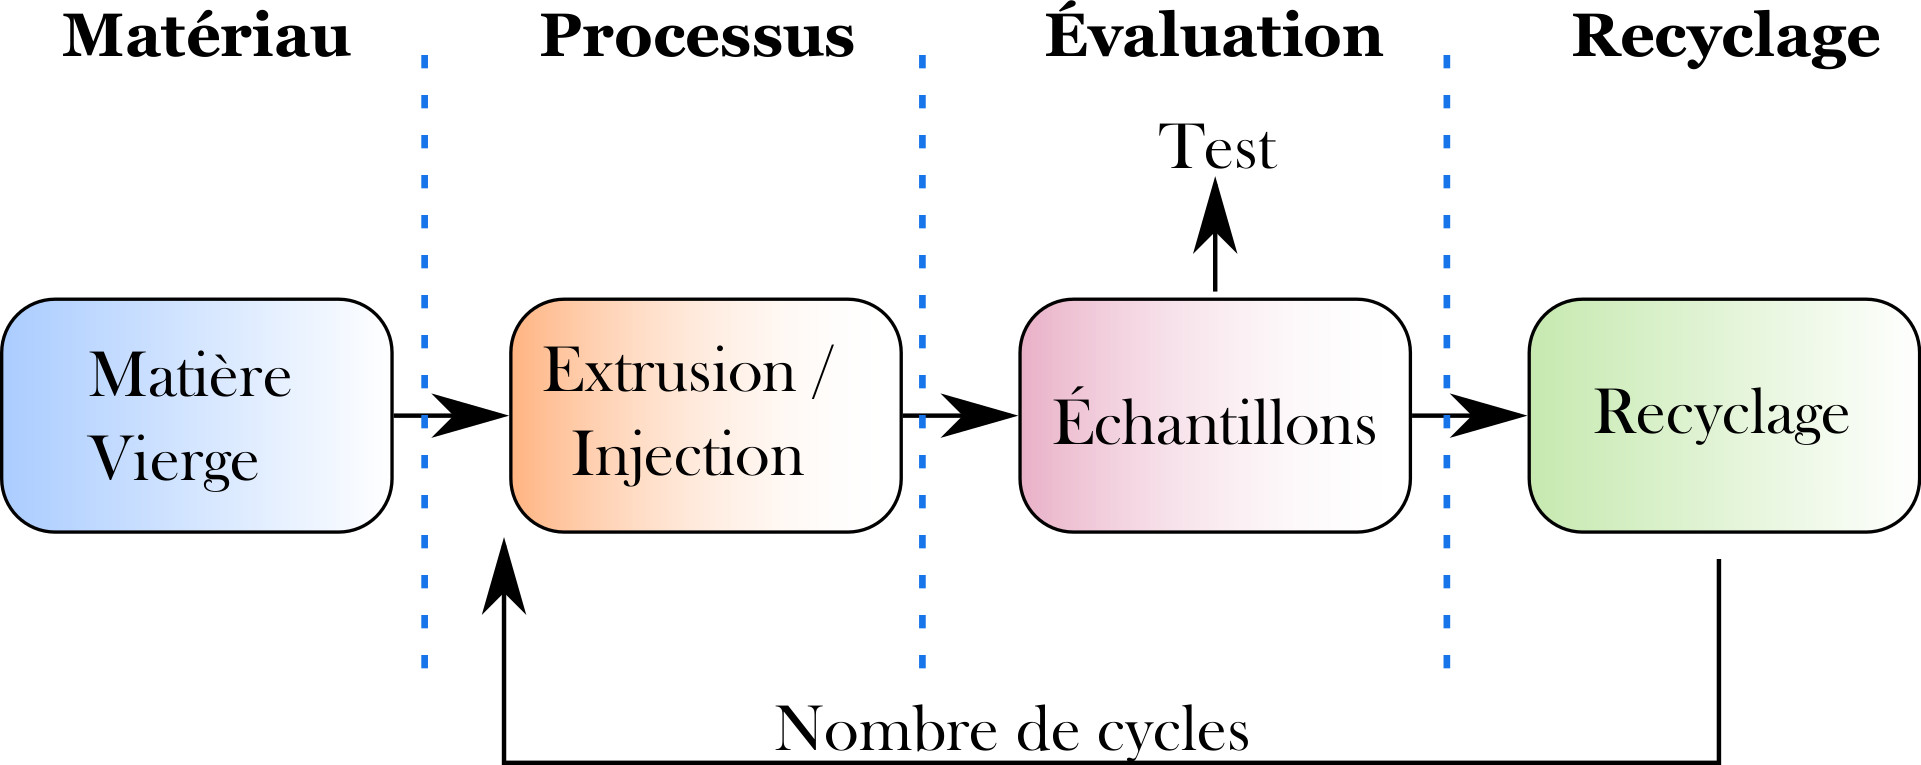
\includegraphics[scale=0.25]{Figures/Chapter-3/Multiple-Processing.pdf}
		\caption{Multiple processing approach for evaluate thermo-mechanical degradation.}
		\label{Chap-3:Fig.Multiple.Processing}
\end{subfigure}
~
\begin{subfigure}[t]{0.49\textwidth}
				\centering
	\includegraphics[scale=0.25]{Figures/Chapter-3/Ageing-Processing.pdf}
	\caption{Methodology for thermo-oxidation degradation.}
	\label{Chap-3:Fig.Ageing.Processing}
\end{subfigure}

\caption{Modelling the Life Cycle of Recycled Polymers. Adapted from \parencite{Vilaplana2008}.}
	\label{Chap-3:Fig.Modelling.Life.Cycle.Recycled.Polymers}
	\end{figure}

The procedures  for modeling the life cycle of recycled plastics can be decomposed the four phases \textit{material}, \textit{process}, \textit{evaluation} and \textit{recycling} (for multiple processing). 
For both cases, \textit{material} is the initial step which has as main goal to characterize the initial condition of the polymer.
% Explaining the figures multiple processing
Figure \ref{Chap-3:Fig.Multiple.Processing} presents the methodology of multiple processing in order to analyze  the structural and morphological changes induced by consecutive processing steps.
	% Explication of the recycling approach
In this sense,  multiple extrusion or injection molding process is a well-tried  approach to assess the recyclability of  polymeric materials  in order to simulate the extended life cycle. 
The main aim of this approach is to have information about the progressive material degradation due to the \textit{process} phase.
In this way, it is possible to optimize the processing conditions during mechanical recycling in order to avoid further degradation.
For example, the choice of temperatures range and/or further addition of stabilizers and other additives are possible options.
% Explaining the methodology of Ageing
On the other hand, figure \ref{Chap-3:Fig.Ageing.Processing} plots the approach for modelling the service life trough different accelerated ageing tests.
% Goal of this
The goal of this test is to mimic accurately the environmental conditions to which polymer materials are exposed during the life service (humidity, temperature, air,  chemical environment -e.g. radiation, biological and microbial attack, pH or salt content-) \parencite{Vilaplana2008}.
Parameters such as temperature, time and type of environment are carefully select to model real conditions.
% Conclusion
In conclusion, these two strategies allow study the degradation processes undergone by synthetic polymers during their first use and sub-sequent mechanical recycling processing. 
Recent approaches have tried to combine reprocessing and accelerated ageing to obtain an overall picture of the extent of the degradation processes that affect the polymers during the entire life cycle \parencite{Vilaplana2008}.
 
% Explaining the framweork of polymer degradation
On the other hand, it is necessary to define the quality characteristics which are assessed in the phase \textit{evaluation} in the model presented in figure \ref{Chap-3:Fig.Modelling.Life.Cycle.Recycled.Polymers}.
These quality characteristics  have to consider  the macro/microscopic properties  in order to fulfill the requirements of manufacturers and consumers, and to guarantee the performance of recycled products in second-market applications \parencite{Karlsson2004}.
% Traditionally
Traditionally in the plastic industry (plastic  producer or processor), the melt flow index (MFI)  is one property that is needed in order to evaluate whether the same process can be used irrespective of whether it uses virgin or recycled polymers. 
This will indicates if it is possible to process the recycled polymeric materials in the same set-up as usual. 
However, several additional properties are needed in order to have a holistic assessment of the  material degradation.
% Proposition of the framework
\textcite{Vilaplana2008,Karlsson2004} developed  a conceptual framework  in order to evaluate the quality assessment of recycled plastics, as detailed in figure \ref{Chap-3:Fig.Quality.Recycling} in three main axes:

\begin{figure}[!htb]
	\centering
	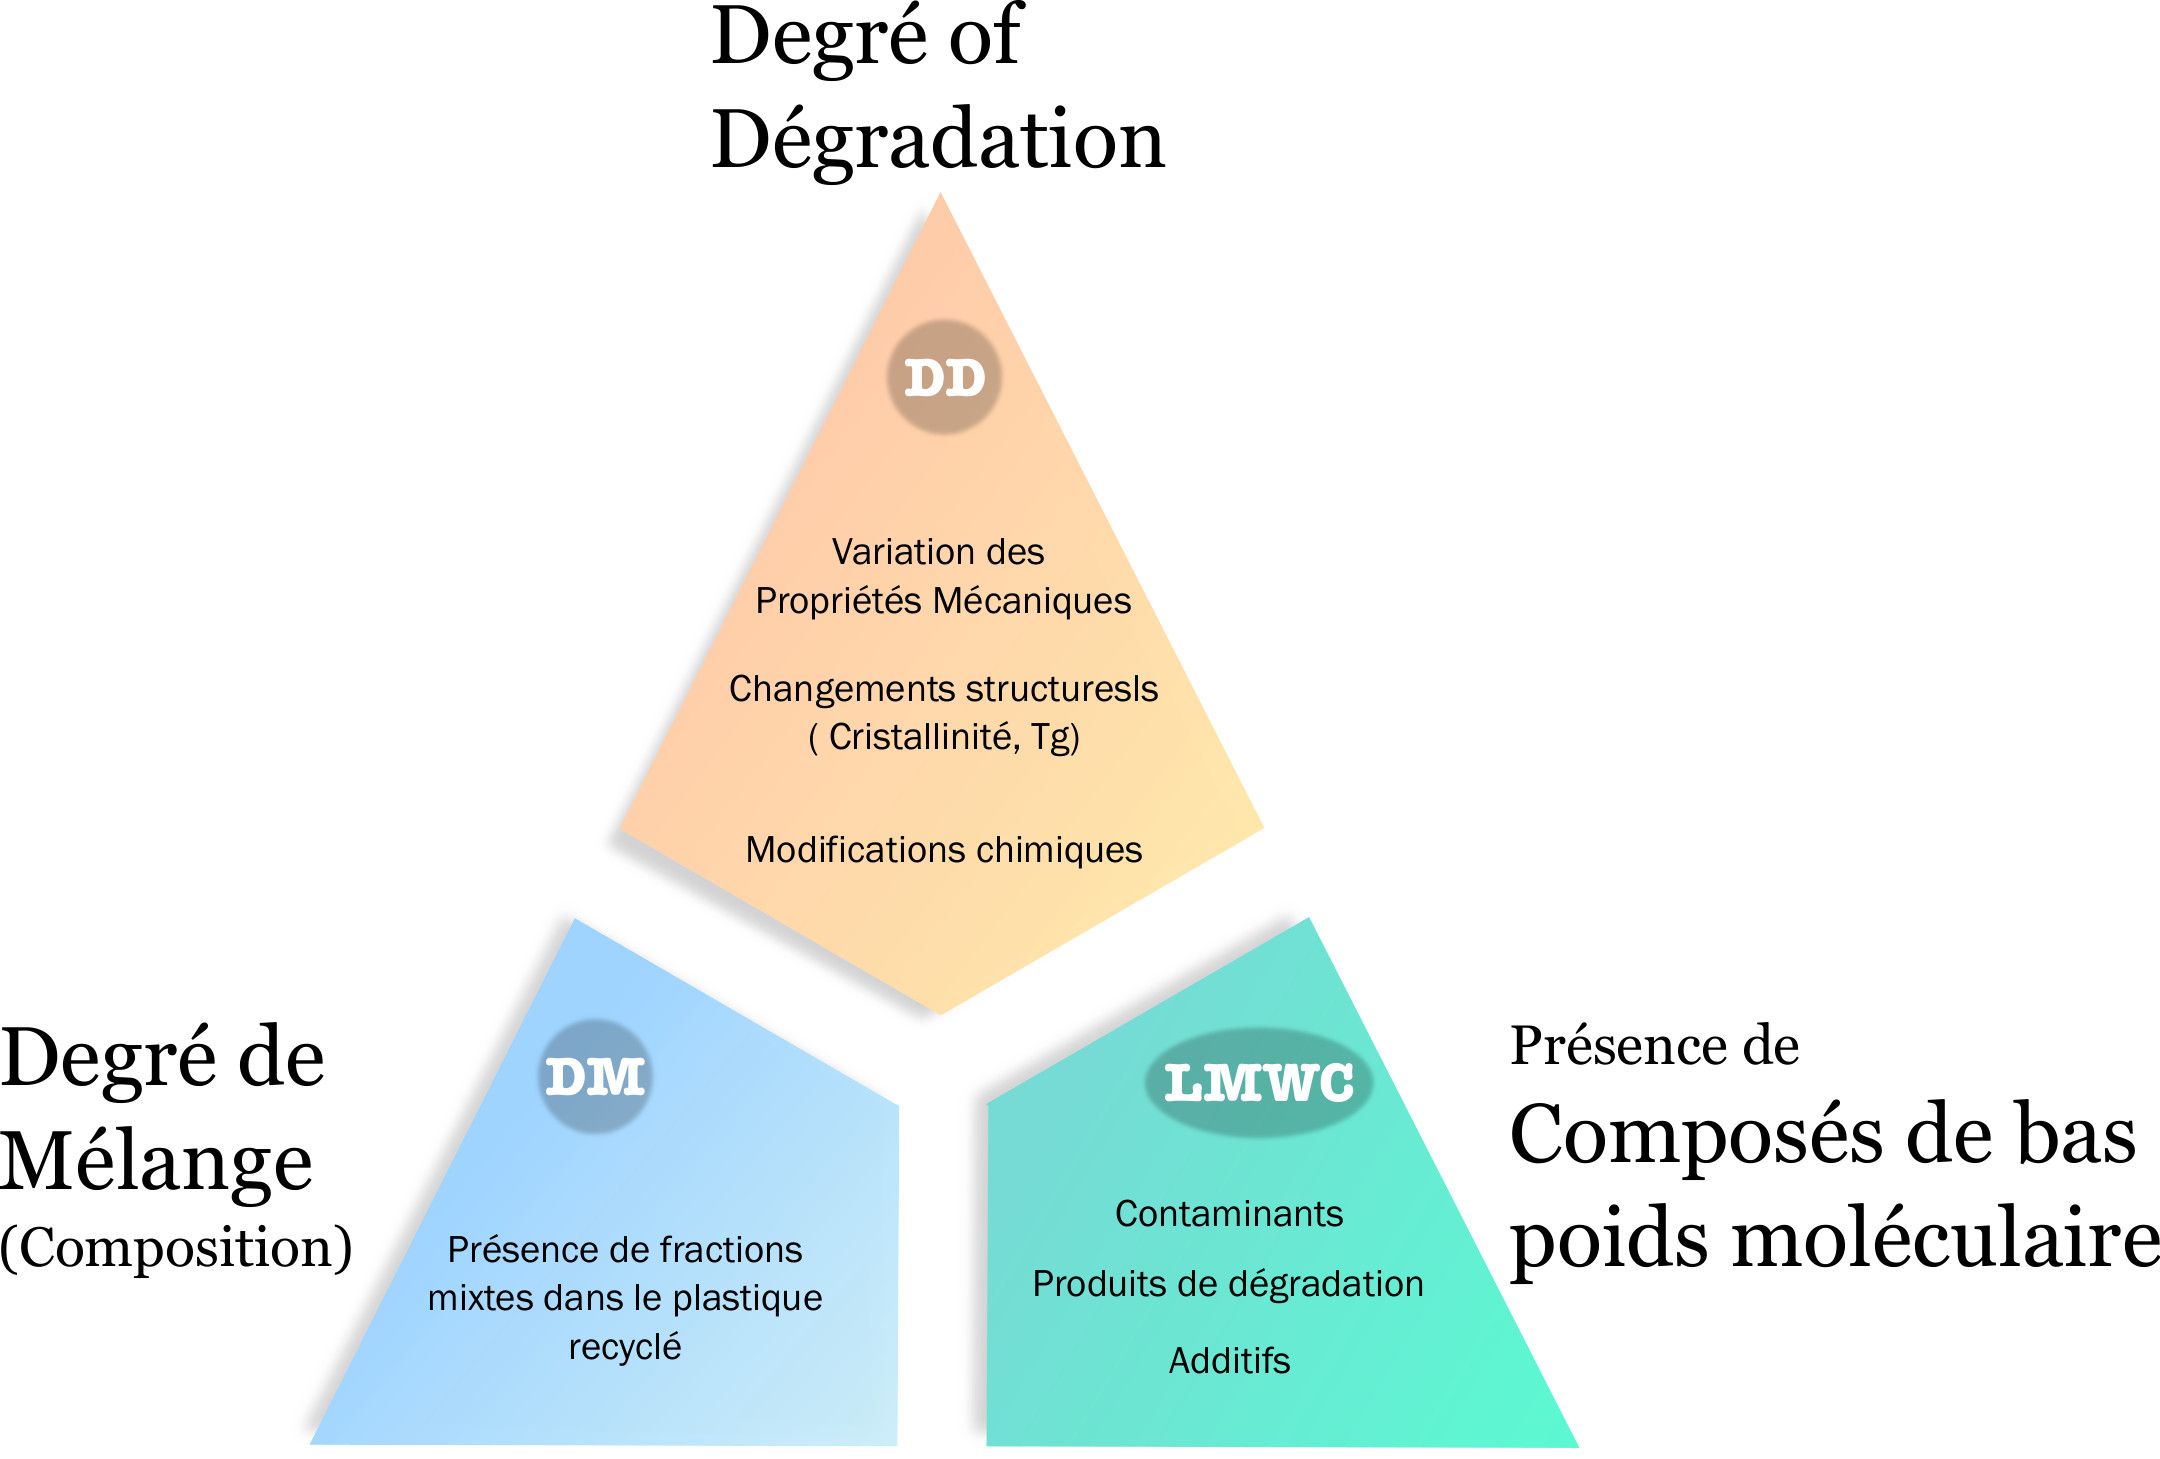
\includegraphics[width=0.7\textwidth]{Figures/Chapter-3/Quality-Recycling.pdf}
	\caption{Key properties for quality assessment of recycled plastics. Adapted from \parencite{Vilaplana2008,Karlsson2004}}
	\label{Chap-3:Fig.Quality.Recycling}
\end{figure}

They can be defined as follows:

	
	\begin{description}[noitemsep]
				\item [\textit{Degree of degradation (DD):}] it determines the evolution of polymer degradation at macro-microscopic scale due to the processing and service life.
	
				\item[\textit{Degree of Mixing (DM):}] it is related to the presence of polymeric impurities  as a consequence of  impure plastic waste streams and poor separation in recycling plant.
		
				\item [\textit{Low molecular weight compounds (LMWC):}] it is related to the presence of additives, contaminants and degradation products in the polymer structure. These element are important in order to fulfill legislation requirements.
	\end{description}
	
% Explaining the logic of this axes
For each axis, there are numerous analytical strategies and characterization tests in order to appropriately  evaluate the degradation of the material.
% Exemple DD
For example, in the category of \textit{degree of degradation (DD)}, the mechanical properties (tensile, compression, flexural strength) are one of the most common measurement of the material quality.
% Exemple DM
Concerning \textit{degree of mixing (DM)}, thermal analysis techniques, and in particular differential scanning calorimetry (DSC), are becoming routine analyses for the characterization of polymer composition
%Exemple LMW
And for \textit{Low molecular weight compounds (LMWC)}, chromatographic techniques such as gas chromatography (GC) and high- performance liquid chromatography (HPLC) are widely employed for the determination of low molecular weight compounds.
Using different detectors such as mass spectrometry (MS), diode-array detector (DAD), and flame ionisation detector (FID), it is possible  the identification and quantification of these analytes.
% Presenting the 
\textcite{Badia2016} present a complete multi-level characterization of recycled polymers as evident in the figure \ref{Chap-3:Fig.Recycling.Test}.
A multi-level scheme in which the different stages of assessment of mechanical recycling performed in lab-scale facilities are represented, along with the analytical techniques commonly used to test the performance and/or degradation state of the resulting material.
% Conclusion
Finally, it depends on the investigator to select the property (or properties) that will be analyzed during the mechanical recycling process.
Therefore, the adequate experimental protocols is implemented. 


\begin{figure}[!hbt]
	\centering
	\includegraphics[width=0.8\textwidth]{Figures/Chapter-3/Recycling-test.pdf}
	\caption{Key properties for quality assessment of recycled plastics. Source  \parencite{Badia2016}}
	\label{Chap-3:Fig.Recycling.Test}
\end{figure}
\newpage

%%  DEFINITION AM
%Additive Manufacturing  is the general name for direct fabrication of prototypes and end-use products using technologies that deposit material layer-by-layer.
%%
%%
%%  PROVIDING  BACKGROUND ABOUT ADDITIVE MANUFACTURING
%% Introduction to AM 
%%There is a considerable interest in the additive manufacturing (AM) technologies because of its capacity of translating virtual solid model data into physical models in a quick and easy process \parencite{Mueller2012}.
%% Introducing the concept of Open source additive manufacturing
%Since the expiration of the \textit{Fused Deposit Modeling} (FDM) patent in the mid-2000s and using a commons-based peer production (CBPP) approach, which is networked-based, modular and collaborative, a new form of AM have been taking place in the recent years with the development of open-source 3D printing \parencite{Kostakis2013, Ford2014}. 
%%	
%%	
%%		%  Definition of AM
%%Additive Manufacturing is the general name for direct fabrication from prototypes (for verification of form, fit and function design) until end-use products using technologies that deposit material layer-by-layer \parencite{ASTM2012,Mueller2012}.
%%		% Introducing the concept of Open source additive manufacturing
%%A new form of AM have been taking place in the recent years with the development of open source 3D printing (OS 3DP) as a results of factors such as commons-based peer production (CBPP) practices (network-based, collaborative, modular approach) in conjunction with the  \textit{Fused Deposit Modeling} (FDM) patent expiration \parencite{ Kostakis2013}.
%%Since the expiration of  \textit{Fused Deposit Modeling} (FDM) patent in the mid-2000s and using a commons-based peer production (CBPP) approach, which is networked-based, modular and collaborative, a new form of AM have been taking place in the recent years with the development of open source 3D printing (OS 3DP). 
%% Exemples of Open Source 3DP
%Projects such as \textbf{RepRap} (or \textbf{Rep}licating \textbf{Rap}id-prototyper) or Fab@Home are extrusion-based systems, they use fused-filament fabrication (FFF) or melt extrusion approach in order to make engineering components and other products from a variety of thermoplastic polymers.
%%
%These type of projects are available to everyone, they  give the chance to (co-)design globally (taking from and contributing to a knowledge commons) and produce locally responding to certain needs\parencite{Malone2007,Bailard2007,Jones2011, HollandDO'DonnellG.Bennett2010a, Kostakis2013}.
%% Importance of OS AM for some communities
%Thanks to the availability of these projects, the fabrication of complex and high-value objects is technically feasible for everyone \parencite{Kostakis2013,Pearce2014k}.  
%Moreover, the cost of the printers themselves has been proven to be economically advantageous for communities like Fablabs, scientific laboratories in the developing world or even schools and middle-class households. 
%%  Applications of OS 3DP
%Furthermore, Open source 3D printers have been proved to be useful tools in different fields such as education \parencite{Kentzer2011a,Schelly2015}, medicine \parencite{Adamatzky2013,He2014,Kasparova2013, DeCiurana2013}, scientific equipment \parencite{Anzalone2013b,Wijnen2014,Leigh2014} and sustainable development \parencite{Pearce2010}. 
%

% 	LOCATE A GAP IN THE RESEARCH




%  DESCRIPTION OF THE PRESENT PAPER
% Goal of the paper

%Contribution of the present research is twofold: first, a general methodology to evaluate the recyclability of polymers used as feedstock of 3D printing machines is proposed. 
%Then, the proposed methodology is applied to the recycling study of the PLA in order to be used by extrusion-based systems using fused filament fabrication (FFF)  which is by now the most adopted technique. 
%Main results of this application contribute to the understanding of the influence of the material physico-chemical degradation on its mechanical properties and then, on its potential distributed recyclability.





%Contribution of the present study is twofold: first,  a general methodology to characterize the recycling of polymers used as 3D printing machines feedstock is proposed.
% Case of application
%Second, the proposed methodology is applied to explore the opportunity to reuse PLA material for open source FFF 3D printers.
% Implications of our study
%which can contribute to understand the physico-chemical degradation characteristics obtained during the whole recycling process.
%In the last part, we conclude with the interest of the methodology and the opportunity to reuse PLA for (FFF) 3D printing.


%\newpage

\section{Methodology to evaluate 3D printing polymer recycling}
\label{Section:General.methodology}


% Connection Recycling - AM 
In recent years, several types of polymer materials have been used in the additive manufacturing (AM) sector in order to produce plastic prototypes \parencite{Guo2013}.
			% Exemples of Open Source 3DP
Projects such as \textbf{RepRap} (or \textbf{Rep}licating \textbf{Rap}id-prototyper) and Fab@Home are \textit{Molten Material} AM systems, which use a fused-filament fabrication (FFF) approach in order to make engineering components and other products from a variety of thermoplastic polymers.
			% Importance of OS AM for some communities
Thanks to the democratization of these projects, the fabrication of complex and high-value products has become accessible for everyone \parencite{Kostakis2013,Pearce2014k}.  
Moreover, the affordable costs of 3D printers can positively impact communities like Fablabs, university laboratories or schools, and open new dimensions to science education that can make a marked impact in developing countries \parencite{Irwin2014}.


%  PRESENTING THE CURRENT RESEARCH FOCUS IN OUR RESEARCH
% Conection of OS 3DP and Recycling
Recently, the adaptation of open-source (OS) 3D printers with domestic waste plastic extruders has been explored as a new prospective approach to polymer recycling in order to prepare 3D printer feedstock material.
	% Consequences of this concept 
The major interest of this approach is the reduction of cost and greenhouse gas emissions related to  waste collection and transportation as well as the environmental impact of manufacturing custom plastic parts.
This distributed polymer recycling approach could be an additional alternative to the conventional centralized polymer recycling \parencite{Baechler2013, Kreiger2014, Anzalone2013, Kreiger2013,Feeley2014}.
% Importance of this approach distributed
Taking into account the significant growing adoption of open-source (OS) 3D printing, distributed polymer recycling approach could be highly relevant as current recycling rates are particularly low. 
		% Open source extruders
Currently, numerous open-source plastic extruders and projects for transforming post-consumer plastic into feedstock for 3D printers have been proposed: 
Lyman Filament Extruder \parencite{Lyman2014}, the Filabot \parencite{McN2012}, Recyclebot \parencite{Baechler2013}, RepRap Recycle Add-on \parencite{Braanker2010}, Precious plastic \parencite{Hakkens2016}, Plastic Bank \footnote{\hyperlink{http://plasticbank.org/}{http://plasticbank.org/}},  Precious plastic \footnote{\hyperlink{http://preciousplastic.com/ }{http://preciousplastic.com/ }} \parencite{Hakkens2016}. 
		% Justification for developing PLA recycling process an OS context
Polylactic Acid (PLA) and Acrylonitrile-Butadiene-Styrene (ABS) filaments, ranging from $1.75$ to $3$ mm of diameter, are the two most common polymers in the open-source (OS) 3D printing context.

		%Economical problematic of filament
From an economical point of view, commercial filament costs are in the range between $\$18.86$ and $\$175.20$ per kg, which is 20 to 200 times above the cost of raw plastic. 
% Literature approving this concept of Distributed polymer recycling
\textcite{Wittbrodt2013, Kreiger2014} proved the economic feasibility for a distributed model with local plastic material recycling (recycled filament) for OS 3D printers in which $1~kg$ of recycled filament was fabricated from about 20 milk jugs for under 10 US cents using the prototype of open-source plastic extruder called ``Recyclebot''.
	% Energy justification
In terms of energy, \textcite{Kreiger2013,Baechler2013} have shown a proof of concept for recycling of high-value polymer waste where savings were between 69\% and 82\% embodied energy for distributed recycling over a centralized recycling approach. 
% Validation of the Interest for recycling for OS 3DP
Therefore, there is an interest in recycling polymeric materials for a 3D printing open-source context.

% 	LOCATE A GAP IN THE RESEARCH
% Establishing the problematic of the article
Therefore,  a first step to study is the physical characterization at the micro and macro level of the recycled material in order to assure new potential uses.
Moreover, the physical characterization is a key element to understand in order to prove the viability of distributed recycling process.
%  Goal of the methodology
The main goal here is to present a generic method to evaluate the opportunity, interest and processes to recycle thermoplastic polymers in order to use them as feedstock for open source 3D printers. 
% Explanation of methodology.
Different aspects have to be studied in order to quantify the degradation of the physical properties of the recycled plastic through 3D printing process chain.
Considering the complexity of the global process  (figure \ref{Complexity.3DP.recycling}), within the framework of the present thesis, the first phase of the recycling process ``Preparation of the Recycled Material'' will not be considered. 
As a second assumption, we consider virgin materials as fully recycled. 



\begin{figure}[!htb]
	\centering
	\includegraphics[width=\textwidth]{Figures/Chapter-3/Methodology/Complexity-3DP-recycling.pdf}
	\caption{ Recycling process for 3D printing adapted from \parencite{Aznar2006} }
	\label{Complexity.3DP.recycling}
\end{figure}

The proposed methodology is shown in (figure \ref{Methodology}). It has been structured in five main steps that will be described as follows: % as it is shown in figure 



\begin{center}
\begin{figure}[p]
	\centering
	\includegraphics[width=\textwidth, height=\textheight, keepaspectratio]{Figures/Chapter-3/Global-Methodology.pdf}
	\caption{Proposed methodology for measuring the degradation of plastic in the chain of 3D Printing}
	\label{Methodology}
\end{figure}
\end{center}
\newpage

\subsection{ Step 1 ``Material definition''}

	%  MATERIAL DEFINITION
	%Goal of  the  "Material Definition"
	The main purpose of this step, called  \textit{\textbf{``Material Definition''}}  (figure \ref{Methodology}),  is to characterize the material to  study.  
	% Recall the polymer characteristics
	The polymer characteristics given by the supplier have to be taken into account for initial establishment of the operating parameters for processing. 
	% Consideration of the POlymer Quantity
	Also, the material quantity needed for the overall experimentation has to be estimated. 
	However, in order to have a real estimation of the material quantity, it is necessary to take into account elements that are defined in subsequent steps.
	The particular elements  to consider in the establishment of the quantity material are:


\begin{itemize}[noitemsep]
	\item The definition by the investigator of the material properties to be studied during the recycling processes (detailed in section \ref{step.processes}).
	\item The quantity of material needed for the fabrication of a single test sample, which is function of the type of test that will be performed.
	\item The definition of the recycling process chains needed  (detailed in section \ref{step.fabrication.of.samples}).
	\item	The definition  of the number  of  recycling cycles that have to be made.
	\item Considerations of the eventual  material loss  during cycles.
\end{itemize}

% Consideration about the intial preparation for processing of the material
Finally, the preliminary preparation stages before  processing must be defined.



%  PROCESS ASSIGNMENT
\subsection{ Step 2 ``Process assignment''}
\label{step.processes}	

This step is divided into two parts: (figure \ref{Methodology})  

\begin{itemize}[noitemsep]
	% Reference process. Selection of the property that it will be study
	\item The \textbf{\textit{``Reference Process''}} refers to the identification of the processes/procedures used for the characterization of the recycled plastic properties.
	Different mechanical, chemical and rheological properties are able to illustrate the polymer degradation \parencite{Vilaplana2007, Vilaplana2008}.
	During this step, the experimenter has to determine his choice, selecting the properties that will be studied through the recycling process.
	
	% Fabrication of the 3DP feedstock
	\item	The \textbf{\textit{``3DP Feedstock Process''}} step refers to the definition of how the feedstock material will be elaborated.
	It is necessary  to specify the different processes that will be used to get the feedstock in usable form for 3D printers. 	
	The different  fabrication parameters of the feedstock material and definition of the material quality obtained are addressed here.		
\end{itemize}



%   FABRICATION OF THE SAMPLES
\subsection{ Step 3 ``Fabrication of samples''}
\label{step.fabrication.of.samples}

% Main goal of the "Fabrication of the samples"
The main goals of the  \textit{\textbf{``Fabrication of Samples''}} step (figure \ref{Methodology})  are:  
%First, to characterize the manufacturing process (\textit{Standard} and the \textit{3D printing}).
%Defining the recycling process chains 
%And second, to define the recycling process chains that are necessary  to characterize the material degradation due to the 3D printing. 


\begin{enumerate}
	% Explaining the manufacturing processes of the samples
	\item Two types of manufacturing processes are proposed in order to compare the material degradation:
	\textit{Standard} and \textit{3D Printing} fabrication. 
	
	\begin{itemize}[noitemsep]
		
		% Explication of the goal of Standard and 3DP processes
		% Goal of the "Standard process"
		\item 	The \textit{``Standard''} process, will serve as reference for the purpose of comparing the obtained results with the 3D printing process. 
		%
		For that reason, it is required to define the equipment and fabrication parameters of the samples using a \textit{Standard} process. 
		%enabling the quality assessment of the recycled material must be defined.
		Therefore, it is necessary to identify the appropriate international standard according to each selected property of the previous step (see \textit{Reference Process}).
		
		% Goal of "3DP process"
		\item 	In the \textit{``3D Printing''} process, the main goals are: first, to characterize the open source 3D printer, and second, to establish the manufacturing parameters of the samples. 
		Literature review about the selected property in the additive manufacturing context can give an initial insight into important parameters to consider.
	\end{itemize}

			% Explication of the "Recycling process chains"
		\item 	 In order to highlight the effects of the different processes on the material, at least four recycling chains are needed to compare the material degradation:
			
			\begin{itemize}[noitemsep]
				% Cycle Reference
				\item \textit{Reference:} used as degradation reference for the recycled material.
				%Cycle of feedstock
				\item	\textit{Feedstock:} used to evaluate the degradation impact due to fabrication of the  feedstock material for the 3D printing machines considered (i.e. filament, pellets, powder...).
				%Cycle of 3DP (reference)
				\item  \textit{3DP (Reference):} used to evaluate the degradation of the material as a consequence of the 3D printing process using the reference equipment.
				%Cycle of 3DP
				\item \textit{3D Printing:} used to evaluate the degradation of the material as a result of the 3D printing process with samples made using a 3D printer with established parameters.		
			\end{itemize} 
	

	
\end{enumerate}

	%   EVALUATION 
	\subsection{ Step 4 ``Evaluation ''}
	
	% Goal of the step: Evaluation
	The goals of the \textit{\textbf{``Evaluation''}} step (figure \ref{Methodology})  are:
	to define the set of variables that describe the targeted properties 	and to describe the selected equipment for the evaluation.
	% Description of the test
	The tests are conducted in order to collect the data according to the international procedures and also considering the entire set of samples according to the recycling process chains (see \textit{Fabrication}).



%  RECYCLING	
\subsection{ Step 5 ``Recycling''}
% Goal of the recycling process
To finish,	the main goal of the  \textit{\textbf{``Recycling''}} process step is to adapt the recycled plastic material for reprocessing.
% Description of Recycling
The recycling process is made individually for each recycling process chain.
% Steps to consider for recycling 
A characterization of the recycling equipment used and a description of the characteristics of the recycled material obtained are made. 



% Concluclusion
%Figure \ref{Methodology} summarizes the proposed methodology.
%\end{enumerate}


%\begin{figure}[H]
%	\centering
%	\includegraphics[scale=0.8]{Figures/Chapter-3/Methodology/Global_Methodology_1.pdf}
%	\caption{Proposed methodology for measuring the degradation of plastic in the chain of 3D Printing}
%	\label{Methodology}
%\end{figure}

In the following sections, we will present the use of this methodology using an case study.

\section{Application case: Recycling PLA for open-source 3D printers}
\label{Section:Application.case}

% Conclusion of this intro
As an application case, in this part we will illustrate the proposed methodology  (section \ref{Section:General.methodology}) by considering the opportunity to recycle one of the thermoplastic materials most widely  used in the open source context: the Polylactic Acid (PLA).
The main interest of using open-source 3D printers is that these systems are the more widely used than any other additive manufacturing system  \parencite{Ford2014}.
We recall that these open-source systems use fused filament fabrication (FFF) approach as working principle.


\subsection{Step 1- Material Definition: PLA}
\label{Subsection.material.definition}
%	% About Bio-polymers
%Moreover, factors such as uncertainty of petroleum supply (and the cost associated), legislation on development of environmentally and economically viable manufacturing and problem of recycling are important drivers for the development of biodegradable plastics and bio-based polymers products. 

%  PROVIDING  BACKGROUND OF PLA
% Introduction of PLA
Polylactic Acid (PLA) is one of the most important bio-based, biodegradable and biocompatible polymers \parencite{Drumright2000,Mohanty2000,Henton2005,Luckachan2011, Soroudi2013}. 
% Definition of the PLA
PLA is a thermoplastic aliphatic polyester obtained from the ring-opening polymerization of lactide, which may be derived from  renewable resources such as potato, starch, sugar cane and corn sugar. \parencite{Agrawal2003,Hamad2013, Castro-Aguirre2016}.
% Aplications of the PLA
PLA offers great promise in a wide range of commodity applications such as bottles, trays, containers and so on. 
Moreover, PLA can be processed by injection molding, blow molding, or be extruded into films, fibers, and sheets
\parencite{Drumright2000,Auras2010, Gupta2007,Lim2008,Lim2010}. 
Therefore, PLA is considered a promising alternative to reduce the municipal solid waste (MSW) disposal issues by offering additional end-of-life scenarios \parencite{Ren2011, Mohanty2002,Mohanty2000,Soroudi2013}. 

%  PROVIDING SPECIFIC DETAILS ABOUT USED MATERIAL 
% Definition of the Material Used in the Experimentation
The selected material for this study was PLA type 4043D, a product of NatureWorks supplied by NaturePlast (Caen, France). 
This material is intended for fabrication of 3D printers feedstock according to the manufacturer's specifications.


\begin{enumerate}[leftmargin=0in,label=\emph{\alph*}.]
	
	% Properties of this PLA
	\item \textit{Initial characterization of the material:}
	
	
	
	The properties of the selected PLA 4043 D are showed in the table \ref{PLA}:

	%\subsubsection*{Characterization of the material}	
	%The selected PLA has a density $1.24 g/cm^3$, tensile yield strength $60MPa$,  tensile modulus of 3600 $MPa$, tensile strength at break $53 MPa$, tensile elongation $6\%$, $MFI=6 g/10min$ at 210\Celsius, a glass transition temperature ($T_{g}$) 55-60\Celsius. 
	
	\begin{table}[H]
		\centering
		\caption{PLA 4043D for open source 3D printing}  
		\begin{tabular}{llll}
			\toprule
			\textbf{Physical Properties}   & \textbf{Value}  & \textbf{Units}     &  \textbf{ASTM Method}    \\  
			\midrule 
			Density & 1.24 &   $gr/cm^{3}$   & D792 \\
			Melt Flow Rate & 6 & $g/10min$ (210\Celsius /$2.16~Kg$  ) & D1238 \\
			Relative Viscosity & 4 & & D5225\\
			Clarity & Transparent & \Celsius & D3418 \\
			Peak Melt Temperature & 145-160& & \\
			Glass Transition Temperature & 55-60 & \Celsius & D3418 \\
			& & & \\
			\toprule
			\textbf{Mechanical Properties}   &   &      &     \\  
			\midrule  
			Tensile Yield Strength & 60 & $ MPa $ &  D882 \\
			Tensile Strength at Break & 53 & $ MPa $ & D882 \\
			Tensile Modulus & 3.6 & $MPa$ & D882 \\
			Tensile Elongation & 6 & \% & D882 \\
			Notched Izod Impact  & 16 & j/m & D256 \\
			Flexural Strength & 83 & $MPa$ & D790\\
			Flexural Modulus & 3.8 & $MPa$ & D790 \\
			Heat Distortion Temperature & 55 & \Celsius    & E2092     \\
			\bottomrule
		\end{tabular}%
		\label{PLA}% 
	\end{table}%
	


	
	
	\item \textit{Estimation of the material quantity:}
	
	We will consider the four recycling process chain as previously defined in section  \ref{Section:General.methodology}.
	One of the criteria was the achievement of at least 8 samples for each cycle in every recycling process chain.
	 It will generate at least $ 4x8x$\textit{(number of cycles)} test samples.
	% Establishing initial mass
	The establishment of the material quantity used in this study will be specified with more details  in the section \ref{Subsection.operational.methodology} once the parameters of the experimentation are defined in the subsequent steps. 

	
%	\subsubsection*{Quantity of material}
	However, a initial estimation can be made.
	The mechanical sample used for this experimentation is according to the standards ISO 527-B as indicated in the figure \ref{mechanical.sample}. 
	It is intended to fabricate 60 samples per cycle, which it is 15 samples per type of recycling process. 
	Therefore, a total of about $\sim 600~gr$ of PLA is a first estimation amount of material to use. 
	However, it is necessary to consider the material that can be lost during the process extrusion and 3DP. Using a security factor of 4 for considering these losses, the amount of material to use is about  $\sim 2400~gr$. 
	
	
	\begin{figure}[!ht]
		\centering
		\includegraphics[scale=1]{Figures/Chapter-3/preparation/mechanical_sample}
		\qquad
		\begin{tabular}[b]{lll}
			\toprule
			\textbf{Parameters } & \textbf{Value } & \textbf{Units} \\
			\midrule
			Volume	& 8017.66	&	$mm^3$			\\
			PLA density 		& 1.24	& $g/cm^3$		\\
			Weight	& 9.9  & $gr$ per sample		\\		
			\bottomrule
		\end{tabular}
		\caption{Mechanical sample according to the standard ISO 527-1B}
		\label{mechanical.sample}
	\end{figure}



	

	% Consideration of the additional degradation
	Appropriate care was taken in order to reduce the material loss between each cycle and also to avoid additional degradation due to environmental conditions.

\newpage	
	\item \textit{Preparation of the material:}
	%  Drying process (Article)
%	Prior to be processed, virgin pellets were uniformly dried during 4h at 80\Celsius in a dehumidifier in order to remove humidity as much as possible.  

	
	%Importance of Polymer drying
One of the important elements to consider in processing PLA is the degradation mechanism via hydrolysis, which is  controlled by the water diffusion in the free volume amorphous phase.
% Reduction of Molar Mass
It exists a concomitant phenomenon associated with molar mass reduction due to the plasticizing effect of the water molecules diffusing into the amorphous region. 
It provokes an increase of the chain segmental motion \parencite{Fambri2010}.
% We have to Dry.
Therefore, the pellets must be dried prior to melt processing to prevent the loss of physical properties. 
Processes that have long residence  times or high temperatures approaching 240\Celsius should dry resins below 50ppm ($0.005\%, w/w$) moisture content in order to achieve maximum retention of molecular weight \parencite{Lim2010}.
% Recommendation of Suppliier
The PLA supplier recommends that resins should be dried to $250ppm$ ($0.025\%, w/w$) moisture content or below before extrusion.
	
% Definition of our case
In the case of this experimentation, PLA is dried by natural convection during $4h$ at $80\Celsius$ in a vacuum drying oven in order to remove humidity as much as possible. 
The material was spread in on aluminum trays in order to increase superficial contact area as it is showed in the figure \ref{secado}.
	
	\begin{figure}[H]
		\centering
		\begin{subfigure}[t]{0.28\textwidth}
		    \centering
			\includegraphics[height=5cm]{Figures/Chapter-3/Horno.png}
			\caption{Vacuum drying oven}
			\label{secado.horno}
		\end{subfigure}
		~
		\begin{subfigure}[t]{0.25\textwidth}
			\centering
			\includegraphics[height=5cm]{Figures/Chapter-3/Drying.jpg}
			\caption{Polylactic Acid pellets}
			\label{secado.pellets}
		\end{subfigure}
		~
		\begin{subfigure}[t]{0.3\textwidth}
			\centering
			\includegraphics[height=5cm]{Figures/Chapter-3/Desecator.jpg}
			\caption{Sealable desiccator for preserving material until processing}
			\label{secado.guardado}
		\end{subfigure}
		\caption{Material preparation before extrusion}
		\label{secado}
	\end{figure}
	
% Conclusion of Drying	
Once the material is dried, it is stored in a sealable desiccator in order to preserve the material from environmental humidity.
	% Consideration of the additional degradation
Appropriate care was taken in order to reduce the material loss between each cycle and also to avoid additional degradation due to environmental conditions.
	
\end{enumerate}



\subsection{Step 2- Processes assignment}
\subsubsection{Step 2.1) Reference process: Mechanical Recycling} 
\label{Sub:Reference.process}


\begin{enumerate}[leftmargin=0in, label=\emph{\alph*}.]
	
	\item  \textit{Identification of the reference process}:

% Recalling the  state of the art presented 	
Based on the general mechanical process and the multiple processing approach for evaluating thermo-mechanical presented in figures \ref{Fig:Mechanical.recycling.steps} and \ref{Chap-3:Fig.Multiple.Processing},
we adapted the general scheme for the particular case of fabrication of recycled filament. 
% Our case
This methodological proposition considers the four recycling chains to compare the material degradation, specified in the methodology section \ref{step.fabrication.of.samples}.
Nevertheless, these four recycling process chains will be explain in more detail the following sections.
Figure \ref{Fig:Mechanical.Recycling.3DP} illustrates the defined approach.
	
	\begin{figure}[H]
		\centering
		\includegraphics[scale=0.4]{Figures/Chapter-3/Mechanical-Recycling-3DP.pdf}
		\caption{Mechanical recycling steps for the case of fabrication of recycled filament. }
		\label{Fig:Mechanical.Recycling.3DP}
	\end{figure}
	
	
%In this preliminary study we don't have to consider the first phase (\ref{mechanical.recycling}). 
% Explaining Materials 
We defined the stage \textit{Material} in the precedent section, making the assumption that we start from virgin materials to perform the recycling process, as stated in the section \ref{Section:General.methodology}.
%
Concerning \textit{Process} stage, we assume that the material will be degraded by these three processes (Injection, Extrusion and 3D printing).
The four recycling chain will allows us to understand and compare the impact of each process in the material degradation.

	
	\item \textit{Definition of the properties to be tested and registered: }

	% Quality polymer recycling
In section \ref{Chap-3:Polymer.Recycling.Background}, we presented a framework with the  three axes for quality assessment of recycled plastics founded in the literature.
Based on this, it is possible to select main parameters/methods in order to assess the quality of the recycled material (\textit{Evaluation} stage of figure \ref{Fig:Mechanical.Recycling.3DP}), 

% Chosing
For our purposes, we selected to analyze the \textbf{\textit{Degree of degradation (DD)}} axis which determines the evolution of polymer degradation at macro-microscopic scale due to the processing and service life \textcite{Vilaplana2008}.
Therefore, mechanical properties will be used as an indicator of the quality of the recycled material.
		
	%  PROVIDING  BACKGROUND PLA RECYCLING
Table \ref{Literature.mechanical.recycling.PLA}  presents a short overview concerning the works of mechanical recycling of PLA in the light of the  axes of quality assessment of recycled plastics
	\parencite{Soroudi2013,Hamad2013}.
% Selection of micro-compounding	
Based on this literature,  we have the first insights about the variation of the mechanical properties for polylactic acid (PLA).
%
On the other hand, injection process, by means of micro-compounding technique, was selected in order to have a reference of degradation.
The characterization of the equipment and the parameters used  are discussed in more detail in section \ref{Sub:Fabrication.samples.reference}. 
	
%	
%	
%	\begin{table}[H]
%		\centering
%		\caption{Overview of mechanical recycling studies of PLA}  
%		
%		\begin{adjustbox}{max width=\textwidth}
%			\begin{tabular}{l|p{2.5cm}p{2cm}cccp{11cm}}
%				\toprule
%				\textbf{Reference}& \textbf{Material}& \textbf{Recycling Process}&  \multicolumn{3}{c}{\textbf{Evaluation}}&  \textbf{Comments}\\ 
%				\cmidrule(lr){4-6}
%				& &  & \textbf{DM}  & \textbf{LMWC} & \textbf{DD} &\\
%				\midrule 
%				
%				%Material valorisation of amorphous polylactide. Influence of thermo-mechanical degradation on the morphology, segmental dynamics, thermal and mechanical performance
%				\textcite{Pillin2008}&PLLA L900 & Injection & & &X &Thermal, mechanical and rheological properties were studied after seven cycles.  \\
%				& & & & & & Oxidative stabilizers were tested in order to evaluate the effect on the recycled material\\ 
%				
%				%Effect of recycling on mechanical behaviour of biocompostable flax/poly(l-lactide) composites
%				\textcite{LeDuigou2008} & PLLA L900&Injection &X & &X& Blends (20\% and 30\% in weight) were made through single extruding process. \\
%				&Flax fibres  &  & & & & Modification of mechanical, thermal, rheological and molecular properties were investigated after six cycles. \\
%				
%				% Characterisation of multi-extruded poly(lactic acid)
%				\textcite{Zenkiewicz2009a} &PLA 2002D &Extrusion&X& &X&Material was recycled ten times using extrusion process. \\
%				& & & & & & Mechanical properties (tensile and impact), melt flow rate, thermal properties and water vapour and oxygen transmission rates were studied  \\
%				
%				% Effect of recycling on rheological and mechanical properties of poly(lactic acid)/polystyrene polymer blend
%				\textcite{Hamad2010}&PLA (ESUN A-1001) &  Extrusion& & &X& Blend of PLA/PS (50/50) was prepared using a single screw extruding process. \\
%				&PS (Sabic 125PS) & & & & & Four recycling cycles were performed by extrusion process. \\
%				& & & & & & Modification on mechanical and rheological properties were explored \\
%				
%				%Recycling Ability of Biodegradable Matrices and Their Cellulose-Reinforced Composites in a Plastic Recycling Stream
%				\textcite{Lopez2011}  & PLLA L9000 &Injection& X& &X& Recycling process of  three commercial bioplastics matrices  is conducted. In all cases, the blend was 30 wt\%. \\
%				& Mater-Bi TF01U/095R& & & & & Mechanical, MFI, and thermal characterization was conducted\\
%				& Mater-Bi YI014U/C & & & & & \\
%				& Cellulosic fibres& & & & & \\
%				
%				%Material valorisation of amorphous polylactide. Influence of thermo-mechanical degradation on the morphology, segmental dynamics, thermal and mechanical performance
%				\textcite{Badia2012b} & PLA 2002D &Injection&X & &X & Characterization on mechanical, thermal properties and segmental dynamics up to five recycling process was studied.\\
%				
%				%Ultrafine particle emissions from desktop 3D printers
%				\textcite{Stephens2013} & PLA / ABS  && & X & & Measurement of the ultrafine particle (UFP) concentration resulting from the operation of two types of desktop 3D printers.\\
%				
%				
%				% Emissions of Nanoparticles and Gaseous Material from 3D Printer Operation
%				\textcite{Kim2015} & PLA / ABS  && & X & & Evaluation of the emission of particulate matter and gaseaous materials during FDM 3D printing\\
%				
%				
%				% Emissions of Ultrafine Particles and Volatile Organic Compounds from Commercially Available Desktop Three-Dimensional Printers with Multiple Filaments
%				\textcite{Azimi2016} & PLA/ABS / HIPS/PCTPE / Nylon/PC  && & X & &Quantification of the emission rates of particles and a broad range of speciated volatile organic compounds (VOCs) from five available desktop FFF 3D printers.  They explore difference in particle and VOC emissions based on filament material and printer characteristics.\\
%				
%				%Characterization of emissions from a desktop 3D printer and indoor air measurements in office settings
%				\textcite{Steinle2016} & PLA/ABS   && & X & & characteristics. Ultrafine aerosol (UFA) emissions and volatic organic compounds (VOC) were measured from a desktop FFF 3D printer. \\
%				
%				
%				\bottomrule
%			\end{tabular}%
%		\end{adjustbox}
%		\label{Literature.mechanical.recycling.PLA}% 
%	\end{table}%
%	
%




\begin{longtabu} to \linewidth [H] {>{\small}X[1,l] >{\small}X[0.5, l] >{\small}X[0.5, l]  >{\small}X[0.1, l] >{\small}X[0.3, l] >{\small}X[0.2, l] >{\small}X[2] }

	\caption{Overview of mechanical recycling studies of PLA}  \\
	
	
			\toprule
			\textbf{Reference}& \textbf{Material}& \textbf{Recycling Process}&  \multicolumn{3}{c}{\textbf{Evaluation}}&  \textbf{Comments}\\ 
			\cmidrule(lr){4-6}
			& &  & \textbf{DM}  & \textbf{LMWC} & \textbf{DD} &\\
			\midrule 
	\endfirsthead

\multicolumn{7}{c}{{\bfseries \tablename\ \thetable{} -- continued from previous page}} \\[0.5mm]			
\toprule
\textbf{Reference}& \textbf{Material}& \textbf{Recycling Process}&  \multicolumn{3}{c}{\textbf{Evaluation}}&  \textbf{Comments}\\ 
\cmidrule(lr){4-6}
& &  & \textbf{DM}  & \textbf{LMWC} & \textbf{DD} &\\
\midrule 
\endhead
			
			
			
			%Material valorisation of amorphous polylactide. Influence of thermo-mechanical degradation on the morphology, segmental dynamics, thermal and mechanical performance
			\textcite{Pillin2008}&PLLA L900 & Injection & & &X &Thermal, mechanical and rheological properties were studied after seven cycles.  \\
			& & & & & & Oxidative stabilizers were tested in order to evaluate the effect on the recycled material\\ 
			
			%Effect of recycling on mechanical behaviour of biocompostable flax/poly(l-lactide) composites
			\textcite{LeDuigou2008} & PLLA L900&Injection &X & &X& Blends (20\% and 30\% in weight) were made through single extruding process. \\
			&Flax fibres  &  & & & & Modification of mechanical, thermal, rheological and molecular properties were investigated after six cycles. \\
			
			% Characterisation of multi-extruded poly(lactic acid)
			\textcite{Zenkiewicz2009a} &PLA 2002D &Extrusion&X& &X&Material was recycled ten times using extrusion process. \\
			& & & & & & Mechanical properties (tensile and impact), melt flow rate, thermal properties and water vapour and oxygen transmission rates were studied  \\
			
			% Effect of recycling on rheological and mechanical properties of poly(lactic acid)/polystyrene polymer blend
			\textcite{Hamad2010}&PLA (ESUN A-1001) &  Extrusion& & &X& Blend of PLA/PS (50/50) was prepared using a single screw extruding process. \\
			&PS (Sabic 125PS) & & & & & Four recycling cycles were performed by extrusion process. \\
			& & & & & & Modification on mechanical and rheological properties were explored \\
			
			%Recycling Ability of Biodegradable Matrices and Their Cellulose-Reinforced Composites in a Plastic Recycling Stream
			\textcite{Lopez2011}  & PLLA L9000 &Injection& X& &X& Recycling process of  three commercial bioplastics matrices  is conducted. In all cases, the blend was 30 wt\%. \\
			& Mater-Bi TF01U/095R& & & & & Mechanical, MFI, and thermal characterization was conducted\\
			& Mater-Bi YI014U/C & & & & & \\
			& Cellulosic fibres& & & & & \\
			
			%Material valorisation of amorphous polylactide. Influence of thermo-mechanical degradation on the morphology, segmental dynamics, thermal and mechanical performance
			\textcite{Badia2012b} & PLA 2002D &Injection&X & &X & Characterization on mechanical, thermal properties and segmental dynamics up to five recycling process was studied.\\
			
			%Ultrafine particle emissions from desktop 3D printers
			\textcite{Stephens2013} & PLA / ABS  && & X & & Measurement of the ultrafine particle (UFP) concentration resulting from the operation of two types of desktop 3D printers.\\
			
			
			% Emissions of Nanoparticles and Gaseous Material from 3D Printer Operation
			\textcite{Kim2015} & PLA / ABS  && & X & & Evaluation of the emission of particulate matter and gaseaous materials during FDM 3D printing\\
			
			
			% Emissions of Ultrafine Particles and Volatile Organic Compounds from Commercially Available Desktop Three-Dimensional Printers with Multiple Filaments
			\textcite{Azimi2016} & PLA/ABS / HIPS/PCTPE / Nylon/PC  && & X & &Quantification of the emission rates of particles and a broad range of speciated volatile organic compounds (VOCs) from five available desktop FFF 3D printers.  They explore difference in particle and VOC emissions based on filament material and printer characteristics.\\
			
			%Characterization of emissions from a desktop 3D printer and indoor air measurements in office settings
			\textcite{Steinle2016} & PLA/ABS   && & X & & characteristics. Ultrafine aerosol (UFA) emissions and volatic organic compounds (VOC) were measured from a desktop FFF 3D printer. \\
			
			
			\bottomrule
	\label{Literature.mechanical.recycling.PLA}% 
		\end{longtabu}%

		
\end{enumerate}




% Proceso de Extrusion
\subsubsection{Step 2.2) 3D Printing Feedstock Process: Extrusion}
\label{Sub:Feedstock.3DP}
% Goal of this step
%The goal of this step is to define how the feedstock materiaL will be obtain. 
% Open source machines justification of the filament
\begin{enumerate}[leftmargin=0in, label=\emph{\alph*}.]
	
	\item  \textit{Manufacturing  process of the 3D printing feedstock material :}
	
		%The goal of this step is to define how the feedstock materiaL will be obtain. 
A considerable number of open source 3D printers  are inscribed in the context of extrusion-based systems, where the loading of material is in form of continuous filament plastic of $1.75-3 mm$ in diameter \parencite{Mueller2012, N.Turner2014}.
		% Justification of Extrusion process
In that respect, extrusion of the polymer into monofilament may be achieved by melt spinning, which is one of  the most important techniques for continuously melt processing of PLA \parencite{Gupta2007, Lim2008}.
For the purpose of this experiment, we will consider this process as a sum of three systems, namely, (I) Feeding system, (II) Extrusion process and (III) Conveyor system, as it can be seen in figure \ref{Extrusion.process.feedstock.3DP}.
		
		
	\begin{figure} [H]
		\centering
		\centering
		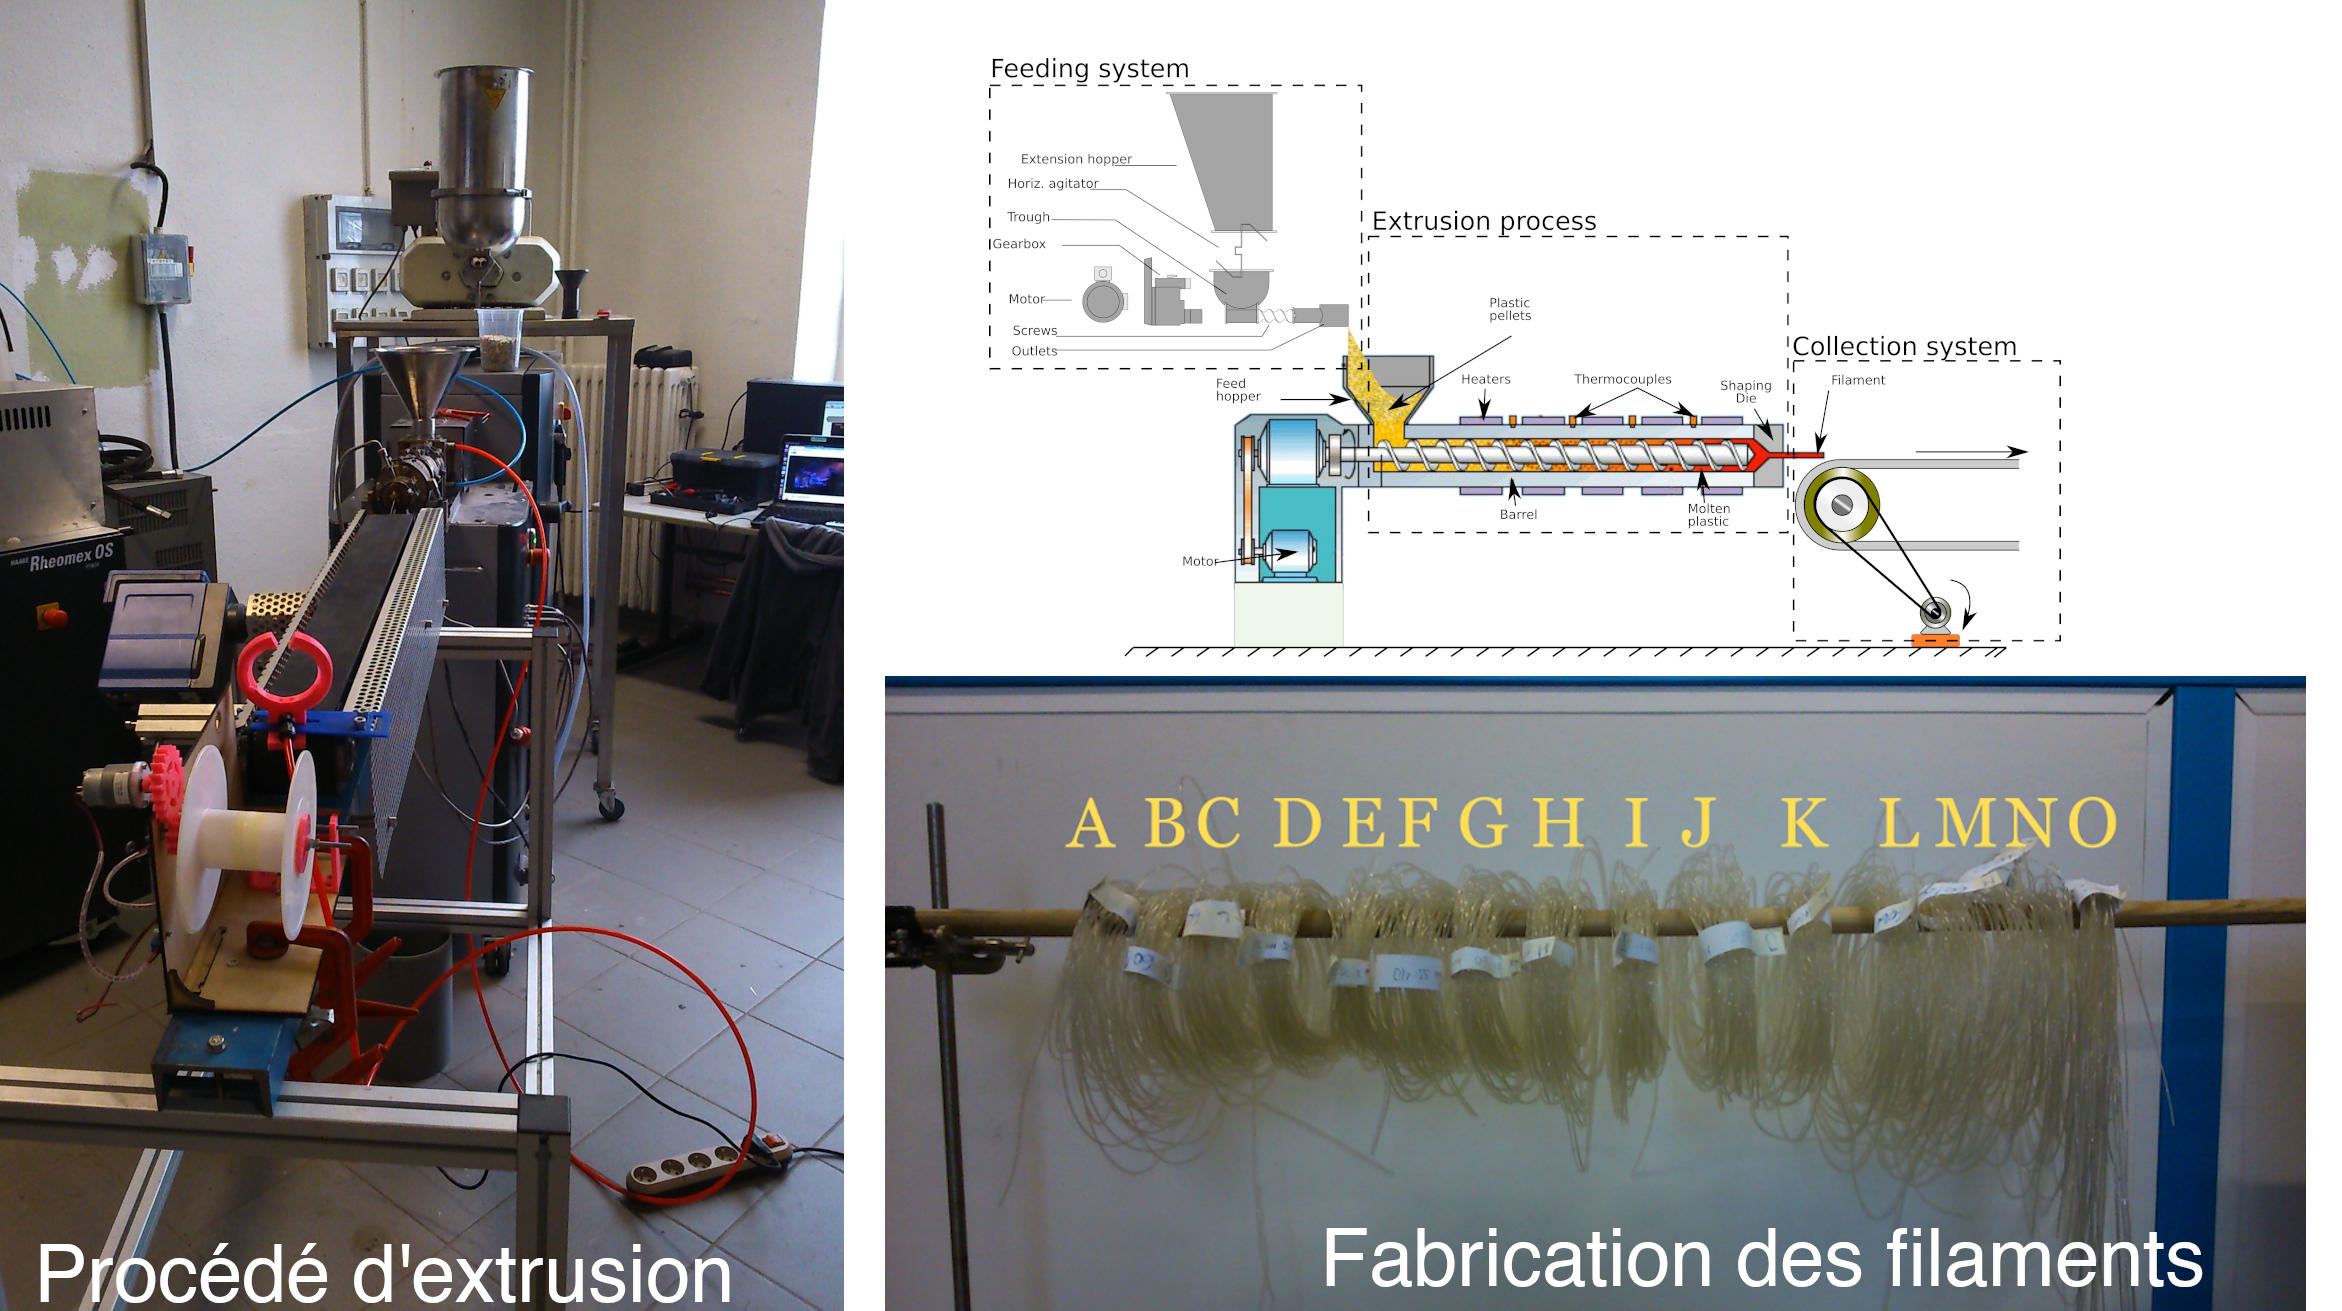
\includegraphics[width=0.7\textwidth]{Figures/Chapter-3/Materials-methods/Process-reference/Extrusion-process.pdf}
		\caption{Schematical extrusion process for fabrication of feedstock 3D printing material}
		\label{Extrusion.process.feedstock.3DP}
	\end{figure}
	
	
	%Explanation of the equipement used in the experimentation
	\item  \textit{Characterization of the experimental conditions:} 
	
		
	
	\paragraph{I. Feeding system}\hfill
	
	\begin{figure} [H]
		\centering
		\includegraphics[scale=0.5]{Figures/Chapter-3/Feeding.png}
		\caption{Schematical view of the feeding system}
		\label{feeding}
	\end{figure}
	
	% Feeding system
The feeding system is performed using a twin screw volumetric feeder  K-TRON (K-MV-KT20). 
All parts in contact with the material being fed are stainless steel. 
The horizontal agitator gently moves the bulk material to the large throat and then into the screws. 
The  material  is transported from the refill system to the hopper onto the feed screw. 
A motor drives the feed screw and the horizontal agitator (screw filler). 
The feed screws transport the bulk material outwards in a constant flow. 
The feed rate is controlled via the speed of the motor and the gearing reduction. 
	
	% Feedrate
Figure \ref{feedrate} shows the calibration curve for pellets PLA. 
The parameters conditions of the feeding system is 100 RPM for the motor using a granulometry of the pellets. 	
The feedrate  used was established at $0.53 \pm0.04~Kg/hr$. 
	
	\begin{figure}[H]
		\centering
	
		\begin{subfigure}[p]{0.6\textwidth}
	\includegraphics[width=0.9\textwidth]{Figures/Chapter-3/Feedrate.pdf}
		\end{subfigure}
~
		\begin{subfigure}[p]{0.3\textwidth}
				\begin{tabular}[c]{ll}
					\toprule
					\textbf{Granulometry} & \textbf{Feedrate}   \\
					&($Kg/h$)  \\
					\midrule
					Pellets	&  $0.53~\pm0.04$				\\		
					\bottomrule
				\end{tabular}
		\end{subfigure}
	
		\caption{Calibration curve for the feeding system}
		\label{feedrate}
	\end{figure}
	
	
	
	
	
	\paragraph{II. Extrusion Process}\hfill
	
	% State of art concerning extrusion process	
Hot Melt Extrusion (HME) process is the most important technique for forming homogeneous PLA. 
The material is heated, molten, pressurized, and forced through a die. 
Commercial grade PLA resins typically  can be processed using a conventional extruder equipped with a general-purpose screw of $L/D$ ratio of 24-30 \parencite{Lim2008,Lim2010}.
	
	
%	Melt rheological properties of PLA have a profound effect on how the polymer flows during extrusion. Since the PLA rheological properties are highly dependent on temperature, molecular weight, and shear rate. Melt viscosities of high molecular weight PLA are on the order of 5000-10000P (500-1000 $Pa.s$) at shear rates of 10-50 $s^{-1}$. These polymer grades are equivalent to $M_{w}$ of ~$100.000~Da$ for injection molding to ~$300.000~Da$ for cast film extrusion applications.
	
	%% Afectacion de las propriedades opticas del PLA
	%The propensity for the lactide monomer to undergo racemization to form \emph{meso}-lactide can impact the optical purity and thus the material properties of the resulting PLA polymer, especially at temperatures above $200$\Celsius \parencite{Lim2010}.
	%%\parencite{Lim2010}
	%Another important screw parameter is the compression ration, which is frequently estimated from the ration of the flight depth in the feed section to th flight depth in the metering section. The recommended compression ration for PLA processing is in the range of 2-3.
	
	
	\begin{figure} [H]
		\centering
		
		\begin{subfigure}[t]{0.6\textwidth}
			\includegraphics[scale=0.6]{Figures/Chapter-3/Extruder.png}
			\caption{Conical counter-rotating twin screw extruder}
			\label{extruder}
		\end{subfigure}
		~
		\begin{subfigure}[t]{0.3\textwidth}
			\includegraphics[scale=0.7]{Figures/Chapter-3/Screw.jpg}
			\caption{\emph{Intensive mixing} screw of the extruder machine}
			\label{screw}
		\end{subfigure}	
		
		\caption{Overview of the extrusion process}
		\label{extrusion.machine}
	\end{figure}
		
% Goal of this process
The extrusion process  is performed in order fabricate the filament used in the process of 3D printing.
			% Definition of the Extrusion system
It was performed using a laboratory scale HAAKE™ Rheomex CTW 100 OS counter-rotating conical twin screw extruder. 
The range speed operation of this machine is between 0-250 $rpm$. The screw speed was set at 60 $rpm$.
The temperature profile selected was 160,170,180\Celsius .

				
Table \ref{parameters.extrusion} shows the important parameters for the extrusion process:
	
	\begin{table}[H]
		\centering
		\caption{Parameters of the extrusion process}
		\begin{tabular}{lcc}
			\toprule
			\textbf{Parameters } & \textbf{Value } & \textbf{Units} \\
			\midrule
			Feeding rate     	& 0.53 	&	$Kg/h$			\\
			Speed collection		& 50-100	& rpm			\\
			Nozzle diameter	          & 1.75  & $mm$		\\
			Rotation speed of extruder	& 30-60 	& $rpm$ 				\\
			Profile temperature  	     & 180/170/160  &	\Celsius			\\
			Granulometry & Pellets - Grinding & \\
			
			\bottomrule
		\end{tabular}
		\label{parameters.extrusion}
	\end{table}
	
	
	\paragraph{III. Conveyor system}\hfill
	
	%Definition of the Conveyor system
	Finally,  a conveyor system was adapted in order to control properly the take-up speed of the filament after extrusion process.	
	A belt conveyor system is used in order to cool  (by natural convection) and to collect the extruded filament.

	The system is made of a metal frame with rollers at either end of a flat metal bed and a belt is looped around each of the rollers. 
	One of the rollers is powered by an electrical motor, which it makes that the belt slides across the solid metal frame bed, moving the filament with a linear speed of collection $v_{lineal}$ which it is function of the rotation speed of the motor $\omega_{motor}$. Figure \ref{conveyor.system} show the schematic model.
	
	
	\begin{figure} [H]
		\centering
		
\begin{subfigure}[t]{0.5\textwidth}
	\includegraphics[width=0.9\textwidth]{Figures/Chapter-3/Conveyor-System.png}
\end{subfigure}
~
\begin{subfigure}[t]{0.45\textwidth}
	\includegraphics[width=0.9\textwidth]{Figures/Chapter-3/Collection_system.png}
\end{subfigure}


		
		\caption{Schematic diagram of the belt conveyor system}
		\label{conveyor.system} 
	\end{figure}
	
	
	
	% Details of the experiment
	
	% Quality parameters for feedstock material
	\item  \textit{Identification of quality parameters feedstock material: }

	% Mechanical properties of the FDM filaments.
	% Punto de Vista mecanico. Importancia de la stiffness
	There are certain elements to consider concerning the requirements for feedstock material for 3D printers.
	From the point of view of mechanical properties, it is necessary to ensure that the filament has certain characteristics such as:  
	
	\begin{itemize}
		\item High flexural modulus and strength to enable continuous spooling and  unspooling operations, 
		\item High compressive strength to not break after passing through the rollers of the 3D printer, and 
		\item High elastic modulus, geometrical and rheological properties in order to be extruded without buckling effect leading to a failure mode of the filament. 
		
	\end{itemize}

The parameter selected for establishing the quality feedstock was diameter regularity ($\phi$). 
This value is an input for our the printing process.
Therefore, a protocol for measuring and the results of this protocol are presented in the results section.

\end{enumerate}


% Results
%The die diameter was 1.65mm and the resulting diameter of filament formed was in the range of 1.78–1.85mm due to the extrudate swelling



\newpage
%Fabrication
\subsection{Step 3- Fabrication of samples} 
\label{Fabrication.samples}

\subsubsection{Step 3.1) Standard: Micro-compounding extrusion and injection molding}
\label{Sub:Fabrication.samples.reference}


\begin{enumerate}[leftmargin=0in, label=\emph{\alph*}.]
	% Identification of International standards for establishing parameters of the process
	\item  \textit{Identification of international standards}: 

	
	This study is focused on \textit{Degree of degradation}  in terms of variation of mechanical properties of the material of the recycled material (See section \ref{Sub:Reference.process}). 
	Therefore, tensile  properties were studied according to ISO 527.
	Tensile specimen is a dog-bone geometry of 150 mm length and central dimensions of 10x4 $mm^2$. 
	
	\item  \textit{Characterization of the equipment:}

	
%  Definition of micro-compounding process as standard.
The Micro-compounding process was selected as our standard manufacturing process.  
It provides a basis for comparison between the different recycled materials.
% Explication of microcompounding
Microcompounders enable to work with a small amount of material (i.e. 3 to 15 g) with the similar processing history as in  conventional twin-screw extruders.


% Description of the Equipement.
The polymer material was processed using a  DSM Xplore intermeshing co-rotating twin screw batch microcompounder with a $5cm^{3}$ capacity. 
The screw diameter of this device tapers from 1 cm to $0.43 cm$ along its $10.75 cm$ length. 


\begin{figure}[H]
	\centering
	\begin{subfigure}[b]{0.19\textwidth}
		\centering
		\includegraphics[width=0.9\textwidth]{Figures/Chapter-3/Compounding_1}
		\caption{Machine}
	\end{subfigure}%
	~ 
	\begin{subfigure}[b]{0.29\textwidth}
		\centering
		\includegraphics[width=0.9\textwidth]{Figures/Chapter-3/Compounding_2}
		\caption{Micro-injection}
	\end{subfigure}
	~ 
	\begin{subfigure}[b]{0.19\textwidth}
		\centering
		\includegraphics[width=0.9\textwidth]{Figures/Chapter-3/Compounding_3}
		\caption{Sample}
	\end{subfigure}%
	~ 
	\begin{subfigure}[b]{0.29\textwidth}
		\centering
		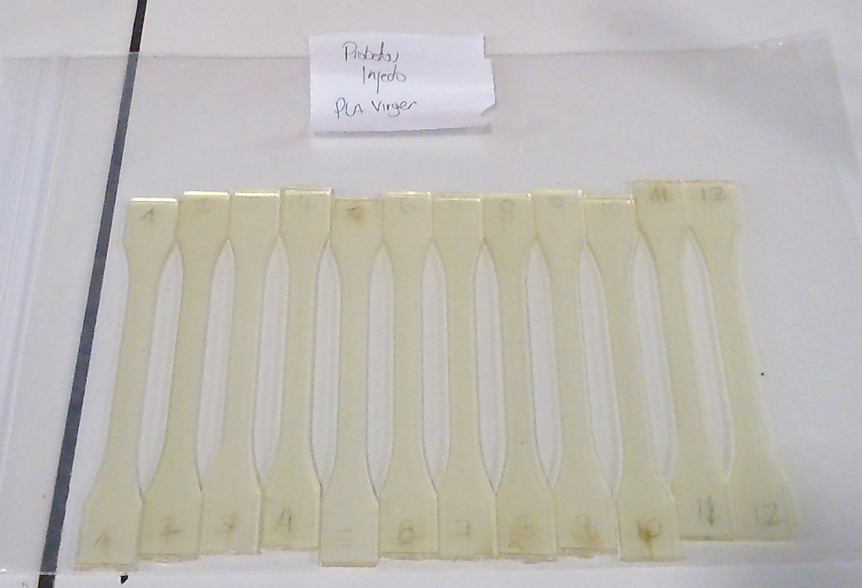
\includegraphics[width=0.9\textwidth]{Figures/Chapter-3/Compounding_4}
		\caption{Samples }
	\end{subfigure}
	\caption{Micro-compounding machine used for fabrication of the mechanical samples}
\end{figure}
	
	\item  \textit{Definition of the operating conditions:}
	
	A constant temperature from the feed throat to the die of 180\Celsius and a screw speed of 100 rpm in co-rotating mode were the parameters adopted. 
	The extruded material was taken  after a mixing time of 3 min.
	The temperatures of the melt and the mold were 190\Celsius and 45\Celsius respectively.   
	The melt was directly injected using the transfer cylinder of DSM Xplore 10 ml injection molding machine  in order to obtain mechanical samples. 
	The injection and holding pressures were set to 9 bars for 30s. 
	Specimens were carefully removed from the mold after 5 min of cooling. 
	Table \ref{parameters.compounding} summarizes the parameters considered for the standard manufacturing process of the samples.

\end{enumerate}


\begin{table}[H]
	\centering
	\caption{Parameters for micro-compounding and micro-injection process}  
	\begin{tabular}{lll}
		\toprule
		\textbf{Parameter}   & \textbf{Value}  & \textbf{Units}  \\  
		\midrule 
		Screw Speed   & 100 &   $rpm$   \\
		Barrel temperature & 180 & \Celsius	 \\
		Mixing time & 3 & $min$ \\
		Injection pressure & 9 & $bar$ \\
		Mold temperature & 45 &  \Celsius \\
		Time of injection & 45 & sec  \\
		\bottomrule
	\end{tabular}%
	\label{parameters.compounding}% 
\end{table}%


\subsubsection{Step 3.2) Fabrication using 3D Printing process: Fused Filament Fabrication (FFF)}
\label{Fabrication:3DP.parameters}

% Goal of this step
The goals of this step are, first, to characterize the open source 3D printer, and second, to establish the manufacturing parameters of the mechanical samples using the OS 3D printer.
%  INTRODUCTION ABOUT CHARACTERIZATION OF THE 3D PRINTER
% Introduction about OS 3DP mouvement
As we stated before in the chapter \ref{Chapter.2}, one of the principal characteristics of open-source 3D printing is that it has been an object of social experimentation, where numerous enthusiasts and communities have developed a significant number of  3D printer machine architectures \parencite{Kostakis2013}. 
% Problem of the high custimization
Therefore, due to the high customization nature, there are different machine architecture configurations which result in inherent variability among different 3D printers.
% Introducing the need of characterize 3DP
It is necessary to characterize the open source 3D printer in order to ensure reproducibility of the printed parts \parencite{CruzSanchez2014}.



\begin{enumerate}[leftmargin=0in, label=\emph{\alph*}.]
	%  DETAILS ABOUT EQUIPEMENT
	% Description of the 3DP Printers
	\item \textit{Characterization of the 3D printing machine:} 
	
	Figure \ref{FoldaRap} presents the two types of 3D printers selected for the fabrication of the samples in this study. 
	They are representative 3D printer among the set of OS machines developed by the RepRap community called \emph{Mondrian} and \emph{FoldaRap} \parencite{Open2015, mondrian2015, CruzSanchez2014}. 
	Indeed, as can be seen in the open-source 3D printer family tree \parencite{Pearce2014k}, they derive from the main branch (XZ Head, Y Bed): Darwin-Sells Mendel-Prusa Mendel. 
	% Dimmensions capacity
	They are a variant of the RepRap machine with a work capability of   $140\times140\times155 (mm^3)$ and  $200\times200\times200 (mm^3)$ for \textit{FoldaRap} and \textit{Mondrian} respectively.  
	% Extrusion system
	The extrusion system can be displaced  in the horizontal plane XY and the heated print bed can be displaced in the vertical direction -Z. 
	% Resolution
	The resolution depicted is in plane $XY = 0.0125 mm$, $Z = 0,00025 mm$ with m5 rods and an accuracy:$0.1 mm$.
	% Plate
	The heated print bed is made of aluminium joined with a Peltier cell and it uses a top layer of kapton in order to improve the adherence of the piece with the print bed.
	
	
	\begin{figure} [H]
		\centering
		\begin{subfigure}[t]{0.45\textwidth}
			\centering
			\includegraphics[scale=0.25]{Figures/Chapter-3/Figure_2}
			\caption{Open Source 3D printer -FoldaRap-}
			\label{FoldaRap}
		\end{subfigure}%
		~ 
		\begin{subfigure}[t]{0.45\textwidth}
			\centering
			\includegraphics[scale=0.5]{Figures/Chapter-3/mondrian}		
			\caption{Open Source 3D printer -Mondrian-}
			\label{mondrian}
		\end{subfigure}
		
		\caption{Open source 3D printers used in the experimentation of the recycled filament}
		
	\end{figure}
	
	%  INTRODUCTION ABOUT PARAMETERS OF FABRICATION
	% Important variable of the 3DP process
	\item \textit{Definition of 3D printing parameters:}
	
	Figure \ref{parameters.3dp} shows the process parameters to be considered in the fabrication of the printed samples. 
	They can be defined as follows:   \parencite{Croccolo2013,Sood2010, Ahn2002}
	
	%!tbp
	\begin{figure} [H]
		\centering
		\includegraphics[scale=0.4]{Figures/Chapter-3/Materials-methods/Fabrication-samples/3DP-cycle/Parameters.pdf}
		\caption{Parameters of the 3D printing process}
		\label{parameters.3dp}
	\end{figure}
	
	
	\begin{itemize}[noitemsep]
		\item \textit{Part building direction}: It refers to the inclination of the part in a build platform with respect to X, Y and Z axis. X and Y-axis are considered parallel to build platform. $Z-axis$ is considered the printing axis.
		\item \textit{Layer thickness:} It is the height of layer deposited by nozzle. It is usually one half of the bead width.
		\item \textit{Bead width (raster width):}It is he width of the filament deposited by nozzle that fills interior regions of part. % Its most common value ranges from $0.3 mm$ to $1 mm$. 
		\item \textit{Fill angle:} It refers to the inclination of the deposited beads of filament with respect to the $x-axis$ of the bulid table. Typical configurations are $90/90$ and $45/45$.
		\item \textit{Air gap:} It is the gap between two adjacent filaments of material on same layer. A zero value means that the rasters touch each other. Positive value means there is a gap. Negative value imply that rasters are overlapped.
		\item \textit{Number of contours:} Defines the number of solid perimeters for the object.
		\item \textit{Nozzle speed:} It is the speed of the printer nozzle when it fabricates the object. (Speed of perimeters, small perimeters, external perimeters, infill – solid, top, bottom layers) 
	\end{itemize}
	
	%  IMPORTANCE OF PARAMETER OF FABRICATION ON ACCURACY
	% Introduction to the characterization  from dimmensional accuracy
	From the point of view of dimensional accuracy, there have been attempts in order to characterize the dimensional performance of the open source 3D printers \parencite{Perez2013,Roberson2013,Johnson2011,CruzSanchez2014}.
	%	Citing my results
From our obtained results in the chapter \ref{Chapter.2}, it was found that according to the International Standard Tolerance Grade of these type of machines could be situated between IT14 and IT16. 
Another conclusion of the chapter \ref{Chapter.2} was that parameters such as layer thickness, raster width and nozzle speed movement can have an impact in the machine accuracy \parencite{CruzSanchez2014}.
	
	%  IMPORTANCE OF PARAMETER OF FABRICATION ON MECHANICAL PROPERTIES
	%  Anisotropy of the mechanical properties in 3DP
	On the other hand, considering the material's mechanical properties in additive manufacturing technology based on extruded-bases systems, one important conclusion of the literature is that there exits anisotropic behavior. It means that the material is directionally dependent.
	% Explication of the anysotropy on 3DP
	Mechanical integrality of the printed part is directly related to factors like the energy adhesion/cohesion between the layers and deposited beads, the growth of the contact area formed between the adjacent beads, the molecular diffusion and randomization of the polymer chains across the interface, and a minimum residence time at elevated temperature in order to assure adequate levels of diffusive bonding \parencite{AtifYardimci1996,Yardimci1997, Agarwala1996,Sun2008}.
	% Elements related with the temperature
	Moreover, the thermal history of interfaces plays an important role in determining the bonding quality. 
	Uneven heating and cooling cycles due to inherent nature of printing process results in stress accumulation in the built part, which it is primarily responsible for week bonding and thus affecting the strength. 
	For that reason, there exist a dependence of the mechanical properties on toolpaths and part orientation.
	% Conclusion of 
	Therefore, mechanical properties are function of parameters of fabrication because they affect meso-structure and fibre-to-fibre bond strength 
	\parencite{Es-Said2000,Ahn2002,Bellini2003, Lee2005,Lee2007, Sood2010,Sood2012,Croccolo2013, Tymrak2014a}.
	
	Finally, taking  into account the factors regarding dimensional and mechanical performances of the 3D printer, figure \ref{specimen.3DP} shows the parameters used in the fabrication of the test samples.
	
	\begin{figure}[H]
		\centering
		
		\includegraphics[scale=0.8]{Figures/Chapter-3/Materials-methods/Fabrication-samples/3DP-cycle/3DP_samples.png}
		\qquad
		\begin{adjustbox}{max width=8cm}
			\begin{tabular}[b]{lcc}
				\toprule
				\textbf{Parameters } & \textbf{Value } & \textbf{Units} \\
				\midrule
				Fill angle					& $0/90 - 45/45$  &		\\
				Bed temperature  	& 60  &	\Celsius			\\
				Nozzle temperature	& 190  & \Celsius		\\
				N° of Contours	& 2 	& 				\\
				Top solid layers		&2	&				\\
				Bottom solid layers		& 2	&			\\
				Fill density					 & 100  & \% 		\\
				Travel speed				& 140  & mm/s		\\
				Nozzle diameter	(FoldaRap)		& 0.5  & mm		\\
				Nozzle diameter	(Mondrian)		& 0.4  & mm		\\
				Bead width 	& \textit{Printer's nozzle}  & mm		\\
				Nozzle speed		& 40  & mm/s		\\
				G-code  & Slic3r & \\
				\bottomrule
			\end{tabular}
		\end{adjustbox}
		
		\caption{Parameters used for fabrication of mechanical samples}
		\label{specimen.3DP}
	\end{figure}
	
\end{enumerate}




\subsection{Step 4- Evaluation: Mechanical properties}
\label{Subsection:Evaluation.PLA}

% Uso de la norma ISO 527
The standard ISO 597 is used in order to determinate tensile properties of the recycled material.  
The specimen used is ISO 527 1B. Table \ref{specimen.measures} shows the respective measurements of this specimen.
This standard covers plastics as filled and unfilled molding, extrusion and cast materials, plastic film and sheets, as well as long fiber reinforced composites.

\begin{figure} [H]
	\centering
	\includegraphics[scale=0.8]{Figures/Chapter-3/Specimen.png}
	\medskip
	%	\begin{adjustbox}{max width=8cm}
	\begin{tabular}[b]{clc}
		\toprule
		& \textbf{Specimen type 1B} & $mm$ \\
		\midrule
		$l_{3}$ & Overall length  &$\geqslant~150$ \\
		$l_{1}$ & Length of narrow parallel-side portion & $60 \pm0.5$ \\
		$r$	& Radius  &	$\geqslant~60$	\\
		$l_{2}$	& Distance between broad parallel-sided portion  &	$106$ to $120$	\\
		$b_{2}$ & Width at ends & $20~\pm0.2$ \\
		$b_{1}$ & Width of narrow portion & $10~\pm0.2$ \\
		$h$ & Preferred thickness & $4~\pm0.2$ \\
		$L_{0}$ & Gauge length & $50~\pm0.5$ \\
		$L$ & Initial distance between grips & $(l_{2})_{0}^{+5}$\\
		\bottomrule
	\end{tabular}
	%	\end{adjustbox}
	\caption{Test specimen measurements}
	\label{specimen.measures}
\end{figure}


% The principle of the test
The principle of this test is performed by elongating a specimen and measuring the load carried by the specimen.
Knowing the specimen dimensions, the load and deflection data can be translated into a stress-strain curve.
The main mains properties that can be extracted from the stress-strain curve are:

\begin{itemize}[noitemsep]
	\item Tensile strength and tensile strength at break ($\sigma_{m}$, $\sigma_{B}$ $[MPa]$)
	\item Tensile strain and nominal strain at break ($\epsilon_{m}$, $\epsilon_{B}$ $[\%]$)
	\item Elastic modulus ($E~[MPa]$)
\end{itemize}


\begin{figure} [H]
	\centering
	\includegraphics[scale=0.7]{Figures/Chapter-3/Diagram.png}
	\caption{Diagram of tensile test}
	\label{mechanical.diagram}
\end{figure}

\emph{Tensile strength} ($\sigma_{m}$) is the maximum tensile stress sustained by the test specimen during the test.
In the case of the \emph{tensile stress at break} $\sigma_{B}$, it is the stress at which the test specimen ruptures. 
The calculation of stress values are based on the initial average original cross-sectional area of the specimen :

\begin{equation}
\sigma= \dfrac{F}{A}
\end{equation}

Where, 

\begin{align*}
\sigma&\qquad  \text{is the tensile stress value in question, expressed in megaspacals [$MPa$]}\\
F& \qquad \text{is the measured force concerned, in newtons $N$}\\
A& \qquad \text{the initial cross-sectional area of the specimen, in $mm^{2}$}
\end{align*}

%Explanation of the variables
On the other hand,  \emph{strain value} ($\epsilon$), is defined as the increase in length per unit original length of the gauge. 
This value can be expressed as a dimensionless ration, or in percentage (\%). 
The \emph{tensile strain} is the corresponding  value of strain at the point  to tensile strength. 
In the same way, \emph{nominal strain at break} is the strain value at the tensile stress at break. 
These values can be calculated as follows:

\begin{align}
\epsilon&= \dfrac{\Delta L_{0}}{L_{0}}\\
\epsilon (\text{\%})&= 100 \times \dfrac{\Delta L_{0}}{L_{0}}
\end{align}

\begin{align*}
\epsilon& \qquad  \text{is the strain value in question, expressed as dimansionless ratio, or in percentage}\\
L_{0}&	\qquad \text{is the gauge lent of the test specimen, in $mm$}\\
\Delta L_{0}&	\qquad \text{is the increase in the specimen length between the gauge marks, in $mm$}
\end{align*}

Finally, the \emph{elastic modulus}$E$ is defined as the ratio of stress (nominal) to corresponding strain below the proportional limit of the material. 
In the diagram of figure \ref{mechanical.machine}, it is the slope in the stress-strain diagram between 0.05\% ($\epsilon_{1}$) and 0.25\% ($\epsilon_{2}$) strain. 
This value can be calculated by secant slope or by linear regression between the strain values $\epsilon_{1}$ and  $\epsilon_{2}$ as it is showed in  figure \ref{elastic.modulus}.

\begin{figure}[H]
	\centering
	\begin{subfigure}[t]{0.36\textwidth}
		\includegraphics[scale=0.6]{Figures/Chapter-3/Modulo1.png}
		\caption{Elastic modulus by secante slope}
		\label{modulo1}
	\end{subfigure}
	\qquad
	\begin{subfigure}[t]{0.36\textwidth}
		\includegraphics[scale=0.6]{Figures/Chapter-3/Modulo2.png}
		\caption{Elastic modulus by regression slope}
		\label{modulo2}
	\end{subfigure}
	\caption{Calculus of the \emph{Elastic modulus} $E$}
	\label{elastic.modulus}
\end{figure}


\begin{enumerate}[leftmargin=0in, label=\emph{\alph*}.]
	%Tensile properties
	
	\item \textit{Selection of parameters:}
	
	The selected parameters then were the tensile strength  ($\sigma_{M}$ \textit{[MPa]}), tensile strain ($\epsilon_{M}$ \textit{[mm/mm]})  tensile stress at break ($\sigma_{B}$ \textit{[MPa]}), strain at break ($\epsilon_{B}$ \textit{[mm/mm]}) and elastic modulus ($E$ \textit{[MPa]}). 
	These parameters can describe the changes in macroscopic mechanical properties of the recycled material.
	
	\item \textit{Characterization of equipment:}
	
% Description of the Apparattus
	An Instron 5569 electromechanical testing machine is used to test material in tension. 
	The drive system moves the crosshead up to apply a tensile load on the specimen using a load cell of 50 KN. 
	
	
	\begin{figure}[H]
		\centering
		\begin{subfigure}[t]{0.6\textwidth}
			\includegraphics[scale=0.6]{Figures/Chapter-3/Machine.png}
			\caption{Universal testing machine}
			\label{mechanical.machine}
		\end{subfigure}
		\hfill
		\begin{subfigure}[t]{0.35\textwidth}
			\includegraphics[scale=0.6]{Figures/Chapter-3/Extensometer.png}
			\caption{Dynamic strain gauge extensometer}
			\label{mechanical.extensometer}
		\end{subfigure}
		\caption{Universal testing machine and dynamic strain gauge extensometer used in the experimentation}
		\label{apparatus}
	\end{figure}
	
	
	The universal testing system showed in figure \ref{mechanical.machine} is composed by a frame that contains the mechanical and electrical components that power the frame, the drive system, and the controller panel.
	%frame
	A rigid, rectangular, load bearing beam from which the ballscrew and guide column extend up to the top plate. 
	%There is a  base adapter that attaches to the center of the base beam. 
	This base Adapter enables a specimen, grip, or fixture to be connected to the base beam.
	%Electrical sistem
	The controller is connected to the frame base where there are a load channel connector (load cell) and two optional strain channel connectors. 
	The controller t makes possible the communication between the transducer (load cell or extensometer) and the computer.
	% Control panel
	A control panel is localized in one of the column and it facilitates performing many of the functions directly at the frame.
	
	%Extensometro
	Figure \ref{mechanical.extensometer} shows a dynamic strain gauge extensometer that is used in order to provide the strain data for the \emph{Modulus-of-Elasticity measurements} and for tensile strain values. The strain error is 0.0001 mm/mm.
	

% Parameters of the apparatus.
Static tensile tests were performed wiht a $50 kN$ load cell. 
%The extensometer was set up with an nominal length of 50 $mm$ to determine elastic modulus. 
	
	
	

\subsubsection{Procedure for mechanical testing}	

The procedure to follow in order to test the mechanical samples are:	

\begin{enumerate}[noitemsep]
	\item Measure of the width and thickness of each specimen.
	\item Place the specimen in the grips of testing machine.
	\item Set the parameters of the testing machine.
	\item Attach the extension indicator.

\end{enumerate}



% Medicion del ancho y espesor de la probeta
The measurement of width and thickness of the specimen is made using a electronic caliper with a resolution of $0.01mm$.
According to the standard, the measurement are made in the center of each specimen and within $5 mm$ of each end of the gage length. In the injection samples, there are draft angles of $1 - 2°$ to facilitate demolding are allowed. Therefore, variations in thickness of up to 0.1 mm are acceptable for the standard specimen of type  1B  ($h_{max}-h) \leq 0.1~mm$. 

\begin{figure}[H]
	\centering
	\begin{subfigure}[t]{0.5\textwidth}
		\includegraphics[scale=1]{Figures/Chapter-3/Caliper.png}
		\caption{Mitutoyo digital caliper used.}
		\label{sample.caliper}
	\end{subfigure}
	\hfill
	\begin{subfigure}[t]{0.45\textwidth}
		\includegraphics[scale=0.6]{Figures/Chapter-3/Measurement.png}
		\caption{Measurement of the width and thickness sample}
		\label{sample.measurement}
	\end{subfigure}
	\caption{Important measurements}
	\label{measurements}
	
\end{figure}

% Colocacion de la probeta en la maquina
Concerning the placement of specimens in the grips of the testing machine, it is necessary to take care to align the long axis of the specimen and the grips with an imaginary line joining the point of attachment of the grips to the machine. A misalignment can produce reduction in the tensile resistance of the samples because of concentration of stress in certain points as it is showed in the figure \ref{sample.alignment}. The distance between the ends of the gripping surfaces are indicated in the \ref{specimen.measures}.

\begin{figure} [H]
	\centering
	\includegraphics[scale=0.8]{Figures/Chapter-3/Alignment.png}
	\caption{Importance of alignment of the samples in the grips}
	\label{sample.alignment}
\end{figure}



% Pre-streeses
Concerning  the setting of tensile machine parameters, 
one of the important parameter to consider in the testing machine is the pre-stress of the sample. 
% Tipical curve sin precarga
In a typical stress-strain curve there is a \textit{toe region}, AC, that does not represent a property of the material.  It is caused by a takeup of slack and alignment or seating of the specimen.
% importancia de la precarga
Small positive pre-stresses ($\sigma_{0}$) are necessary to avoid a toe region (figure \ref{sample.toe}) at the start of the stress/strain diagram.  
This definition ensures a repeatable starting point of the test which is quite independent from operator or equipment influences.

\begin{figure}[H]
	\centering
	\begin{subfigure}[t]{0.45\textwidth}
		\includegraphics[scale=0.8]{Figures/Chapter-3/Toe.png}
		\caption{TOE region in a typical stree-strain diagram.}
		\label{sample.toe}
	\end{subfigure}
	\qquad
	\begin{subfigure}[t]{0.45\textwidth}
		\includegraphics[scale=0.8]{Figures/Chapter-3/Prestress.png}
		\caption{Positive pre-stresses ($\sigma_{0}$)in order to avoid a toe region}
		\label{prestress}
	\end{subfigure}
	\caption{Pre-stress in order to avoid toe region}
	\label{toe}
\end{figure}


The pre-stresses ($\sigma_{0}$)  shall not exceed the following value:

\begin{align}
\mid\sigma_{0}\mid & \leqslant 5x10^{-4}E_{t}, &\text{for modulus measurement}\\
\sigma_{0} &\leqslant 10^{-2}\sigma_{m}, &\text{for relevant stresses} 
\end{align}

In the case of this experimentation, the value of pre-stress has been set to $\sigma_{0}=0.5~MPa$ in order to obtain both, modulus and stresses measurements.


% Ubicacion del extensometer

Once it is balanced the prestresses, it is necessary to attach the extensometer in the center of the sample as it is showed in the figure \ref{setting.extensometer}. The initial gauge length is $50mm$.

\begin{figure} [H]
	\centering
	\begin{subfigure}[t]{0.35\textwidth}
		\includegraphics[scale=1]{Figures/Chapter-3/Procedimiento_extensometro.jpg}
		\caption{Extensometer in the specimen}
		\label{procedure.extensometer}
	\end{subfigure}
	\qquad
	\begin{subfigure}[t]{0.4\textwidth}
		\includegraphics[scale=0.7]{Figures/Chapter-3/Marks.jpg}
		\label{marks}
		\caption{Marks in the samples in order to attach the extensometer}
	\end{subfigure}
	\caption{Setting up the extensometer in the mechanical sample}
	\label{setting.extensometer}
\end{figure}

% Speed of testing
In the matter of speed of testing, $v$, which is the rate of separation of the grips of the testing machine. 
It is tipically  established a range between $0.125-0.75~mm/min$ for calculation of the elastic modulus and 5 or 50mm/min for measuring strength and elongation.
For the purpose of this experimentation, a speed of testing value of $1mm/min$ is established.

%Conditioning
Concerning the observance of defined conditioning and ambient conditions with regard to temperature and humidity is of great importance with regard to the comparability of test results.
The tests are carried out in a \textit{standard atmosphere},  as specified in ISO 291 and presented in table \ref{atmospheric}.

\begin{table}[H]
	\centering
	\caption{Standard conditions}
	\begin{tabular}{lcc}
		\toprule
		\textbf{Parameter } & \textbf{Value } & \textbf{Units} \\
		\midrule
		Temperate atmosphere & $23\pm2$	& \Celsius 			\\
		Relative humidity & $50\pm10$   & \%		\\	
		\bottomrule
	\end{tabular}
	\label{atmospheric}
\end{table}


As previously stated,  it is necessary to consider the amount of moisture absorbed by the polymer from atmosphere conditions \parencite{Henton2005}.
Therefore procedure is  to keep specimens in a  standard temperature and inside of sealable desiccator in order to preserve the material from environmental humidity for at least 48 hours prior to the test.

	
	

	
	
	\item \textit{Collection of results:}
	
	Once the specimens are tested, the table \ref{Table.mechanical.results} is proposed in order to collect  the necessary data for further statistical analysis for each recycling process chains.
	
	
	% Table generated by Excel2LaTeX from sheet 'Feuil1'
\begin{longtabu} to \linewidth [H] { >{\small}X[1,l] >{\small}X[1, l] >{\small}X[1, l]  >{\small}X[2, l] }

		\caption{Database of mechanical results used in the experimentation.}\\

				\toprule
				\textbf{Type of information} &  \textbf{Parameters}    & \textbf{Units} & \textbf{Observations} \\
				\midrule
\endfirsthead		

\multicolumn{4}{c}{{\bfseries \tablename\ \thetable{} -- continued from previous page}} \\[0.5mm]			
				\toprule
				\textbf{Type of information} &  \textbf{Parameters}    & \textbf{Units} & \textbf{Observations} \\
				\midrule
\endhead		

\midrule 
\multicolumn{4}{|r|}{Continued on next page.}\\
\midrule
\endfoot

		
\endlastfoot			
				
Identification 	& Initial quantity & ($gr$)      &  \\
		of material		& Drying &  \textit{dd/mm/yyyy}     & Date and conditions of drying. \\
				\midrule
										& Sample & $1,2,3...$      &  \\
				& Recycling process chain &  Ref/3DP/ Feed/3DP(Ref)     & Type of recycling process chain    \\
	Description & Degradation &   One - Five    & Number of cycles of the sample \\
		of the		& Thickness & (mm)  &  \\
		sample		& Width & (mm)  &  \\
				& Area  & ($mm^{2}$) &  \\
				& Weight & ($gr$)  &  \\
				\midrule
	& Profile Extrusion &      & Torque and nozzle pressure profile in the extrusion process. \\
Description				& Collection Speed &       &  Collection speed used for recollection of the filament\\
 of the			& Diameter measurement &  $mm$     & Diameter of filament  \\
	3DP feedstock  material					& Fill angle & $45/45 - 0/90$   & \\
		(Only for 3DP samples)			& Date of sample & \textit{dd/mm/yyyy}      & Date of fabrication of printed sample \\
				\midrule
				\multirow{5}{*}{Description of the test} 	& Date of test &  \textit{dd/mm/yyyy}     &  \\
				& Speed & (mm/min) &  \\
				& Pre-stress  & (MPa) & \\
				& Validity & Yes / No &  \\
				& Comments &       &  \\
				\midrule
				& Young &  $E$ (MPa) &  \\
				& Tensile load & $L$ (N)   &  \\
				& Tensile strength &$\sigma_{M}$ (MPa) &  \\
				& Tensile elongation & $Elo$ (mm)  &  \\
Mechanical		& Tensile strain & $\epsilon_{M}$  (mm/mm) &  \\
				& Tensile load at break & $L_{B}$ (N)   &  \\
Properties			& Tensile elongation machine at break & (mm)  &  \\
				& Tensile stress at break & $\sigma_{B}$ (MPa) &  \\
				& Tensile elongation at break & $Elo_{B}$ (mm)  &  \\
				& Nominal strain at break & $\epsilon_{B}$  (mm/mm) &  \\
				\bottomrule
		\label{Table.mechanical.results}%
			\end{longtabu}%
			
	
	
	
\end{enumerate}



\subsection{Step 5- Recycling process: Plastic shredding}

%  Goal of this step and justification
Size reduction of the samples of each recycling cycle is required in order to reprocess the material.

%!tbp
\begin{figure} [H]
	\centering
	\includegraphics[scale=1]{Figures/Chapter-4/degradation/recycling/recycling}
	\caption{Machine used for the recycling process}
	\label{recycling}
\end{figure}



\begin{enumerate}[leftmargin=0in, label=\emph{\alph*}.]
	% Equipement
	\item \textit{Operational conditions of the recycling process: }
	
	A cutting mill machine SM 300 Retsch\textsuperscript{\textregistered}  with a selectable speed range from 700 to 3,000 $rpm$ was used.  
	The selected speed was 700 $rpm$.
	
	\item \textit{Granulometry of recycled material:}
	
	The final fineness achieved was in a range of $0.2-2~mm$.
	%The selected speed rotation was 700$rpm$. 
\end{enumerate}


\subsection{Experimental strategy}
\label{Subsection.operational.methodology}
%Explication of the recycling process chains
Figure \ref{Operational.methodology} resumes the followed experimental strategy in order to compare the material degradation of the four proposed recycling process chains : \textit{Reference, Feedstock, 3DP reference} and \textit{3DP evaluated} (horizontal axis of Figure \ref{Operational.methodology}) as explained in section \ref{step.fabrication.of.samples}.
%Explication of operational steps
Then, for each recycling process chain, the initial material, have been reprocessed using the operational steps (vertical axis Figure \ref{Operational.methodology}) until 5 recycling cycles have been reached. Each recycle process chain is described in terms of the operational steps (\textit{A,B,C...}) to be followed in order to deploy the global recycling process.

% Considering the material quantity knowing that there are elements that I defined already
On the other hand, a more accurate estimation of the material quantity requirement can be made at this point. Considering that the properties to be studied, equipment of reference, 3D printing process and the quantity of the cycles are clearly defined.  
% and the criteria of samples established in section \ref{Subsection.material.definition}
In preliminary attempts, the loss of material was estimated in the micro-compunding process as  $\sim50gr$, and for the plastic shredding as $\sim30gr$.
Therefore, a initial mass of $500~gr$ for the Reference was established.   
Regarding to extrusion process, the losses of material were about $\sim200gr$. 
As a consequence, a initial mass of $3kg$ was established for the others recycling process chains (3D Printing (Evaluated), Feedstock and 3DP (Reference)).




\begin{figure}[H]
	\centering
	\includegraphics[scale=0.8]{Figures/Chapter-3/Methodology/Global_Methodology_2.pdf}
	\caption{Operational  steps using the methodology of recycling}
	\label{Operational.methodology}
\end{figure}



\section{Conclusion}

% Revisiting the Goal of the Paper from the Intro
% Goal of the paper
In this chapter, we propose a general methodology to characterize the recycling of polymers  used 	as feedstock for open source 3D printing machines.
%
This general methodology was proposed based on the literature of polymer recycling.
%
The definitions of polymer degradation,  types of  degradation  and methods/tools for assessing the quality material were presented.
% Case of application
The proposed methodology was applied to study the conditions for reusing polylactid acid (PLA), which is a material widely used in the context of open source 3D printing using the fused filament fabrication (FFF) technique. 
%
The mechanical properties of the recycled material (\textit{Degree of Degradation -DD-}) were selected as an estimator of the material degradation.
we have to highlight that these mechanical properties represent only a partial evalutaion of the material. Nevertheless, we selected this properties because in a large perspective, we have to define if the recycled material is resistant enough to the mechanical solicitations.
Starting from this base, it will possible to study later other characteristics such as the changes in the micro-structure properties, or even in the change in the manufacturing conditions of the feedstock and printing parts.


%Selection of Lab Machines
On the other hand, in our study we decided to use laboratory machines. 
As stated in the chapter \ref{Chapter.1} section \ref{Chap-1:Paragraph.II.RQ2}, there have been some contributions to the development of open-source extruder systems (Lyman Filament Extruder \parencite{Lyman2014}, Filabot \parencite{McN2012}, Recyclebot \parencite{Baechler2013}, RepRap Recycle Add-on \parencite{Braanker2010}, Precious plastic \parencite{Hakkens2016}).
However, we decided to use laboratory systems that allow us to ensure the reproducibility of the conditions  for recycling. 
These recycling conditions from a laboratory experiment enable to have a first reference model for comparing to other extrusion processes.
Therefore, it is interesting to replicated the presented methodology using an open-source extruder machine in order to observe the difference in the material degradation.
Also, it is interesting to qualify this OS machines acknowledging that there is a difference in terms of cost, performance and reliability of the open-source versus commercial extruders. 

In the next chapter, the results of this case study will be presented.

%\printbibliography
